\documentclass[12pt,]{krantz}
\usepackage{lmodern}
\usepackage{amssymb,amsmath}
\usepackage{ifxetex,ifluatex}
\usepackage{fixltx2e} % provides \textsubscript
\ifnum 0\ifxetex 1\fi\ifluatex 1\fi=0 % if pdftex
  \usepackage[T1]{fontenc}
  \usepackage[utf8]{inputenc}
\else % if luatex or xelatex
  \ifxetex
    \usepackage{mathspec}
  \else
    \usepackage{fontspec}
  \fi
  \defaultfontfeatures{Ligatures=TeX,Scale=MatchLowercase}
    \setmonofont[Mapping=tex-ansi,Scale=0.7]{Source Code Pro}
\fi
% use upquote if available, for straight quotes in verbatim environments
\IfFileExists{upquote.sty}{\usepackage{upquote}}{}
% use microtype if available
\IfFileExists{microtype.sty}{%
\usepackage{microtype}
\UseMicrotypeSet[protrusion]{basicmath} % disable protrusion for tt fonts
}{}
\usepackage{hyperref}
\PassOptionsToPackage{usenames,dvipsnames}{color} % color is loaded by hyperref
\hypersetup{unicode=true,
            pdftitle={Explanatory Model Analysis},
            pdfauthor={Przemyslaw Biecek and Tomasz Burzykowski},
            colorlinks=true,
            linkcolor=Maroon,
            citecolor=Blue,
            urlcolor=Blue,
            breaklinks=true}
\urlstyle{same}  % don't use monospace font for urls
\usepackage{natbib}
\bibliographystyle{apalike}
\usepackage{color}
\usepackage{fancyvrb}
\newcommand{\VerbBar}{|}
\newcommand{\VERB}{\Verb[commandchars=\\\{\}]}
\DefineVerbatimEnvironment{Highlighting}{Verbatim}{commandchars=\\\{\}}
% Add ',fontsize=\small' for more characters per line
\usepackage{framed}
\definecolor{shadecolor}{RGB}{248,248,248}
\newenvironment{Shaded}{\begin{snugshade}}{\end{snugshade}}
\newcommand{\AlertTok}[1]{\textcolor[rgb]{0.94,0.16,0.16}{#1}}
\newcommand{\AnnotationTok}[1]{\textcolor[rgb]{0.56,0.35,0.01}{\textbf{\textit{#1}}}}
\newcommand{\AttributeTok}[1]{\textcolor[rgb]{0.77,0.63,0.00}{#1}}
\newcommand{\BaseNTok}[1]{\textcolor[rgb]{0.00,0.00,0.81}{#1}}
\newcommand{\BuiltInTok}[1]{#1}
\newcommand{\CharTok}[1]{\textcolor[rgb]{0.31,0.60,0.02}{#1}}
\newcommand{\CommentTok}[1]{\textcolor[rgb]{0.56,0.35,0.01}{\textit{#1}}}
\newcommand{\CommentVarTok}[1]{\textcolor[rgb]{0.56,0.35,0.01}{\textbf{\textit{#1}}}}
\newcommand{\ConstantTok}[1]{\textcolor[rgb]{0.00,0.00,0.00}{#1}}
\newcommand{\ControlFlowTok}[1]{\textcolor[rgb]{0.13,0.29,0.53}{\textbf{#1}}}
\newcommand{\DataTypeTok}[1]{\textcolor[rgb]{0.13,0.29,0.53}{#1}}
\newcommand{\DecValTok}[1]{\textcolor[rgb]{0.00,0.00,0.81}{#1}}
\newcommand{\DocumentationTok}[1]{\textcolor[rgb]{0.56,0.35,0.01}{\textbf{\textit{#1}}}}
\newcommand{\ErrorTok}[1]{\textcolor[rgb]{0.64,0.00,0.00}{\textbf{#1}}}
\newcommand{\ExtensionTok}[1]{#1}
\newcommand{\FloatTok}[1]{\textcolor[rgb]{0.00,0.00,0.81}{#1}}
\newcommand{\FunctionTok}[1]{\textcolor[rgb]{0.00,0.00,0.00}{#1}}
\newcommand{\ImportTok}[1]{#1}
\newcommand{\InformationTok}[1]{\textcolor[rgb]{0.56,0.35,0.01}{\textbf{\textit{#1}}}}
\newcommand{\KeywordTok}[1]{\textcolor[rgb]{0.13,0.29,0.53}{\textbf{#1}}}
\newcommand{\NormalTok}[1]{#1}
\newcommand{\OperatorTok}[1]{\textcolor[rgb]{0.81,0.36,0.00}{\textbf{#1}}}
\newcommand{\OtherTok}[1]{\textcolor[rgb]{0.56,0.35,0.01}{#1}}
\newcommand{\PreprocessorTok}[1]{\textcolor[rgb]{0.56,0.35,0.01}{\textit{#1}}}
\newcommand{\RegionMarkerTok}[1]{#1}
\newcommand{\SpecialCharTok}[1]{\textcolor[rgb]{0.00,0.00,0.00}{#1}}
\newcommand{\SpecialStringTok}[1]{\textcolor[rgb]{0.31,0.60,0.02}{#1}}
\newcommand{\StringTok}[1]{\textcolor[rgb]{0.31,0.60,0.02}{#1}}
\newcommand{\VariableTok}[1]{\textcolor[rgb]{0.00,0.00,0.00}{#1}}
\newcommand{\VerbatimStringTok}[1]{\textcolor[rgb]{0.31,0.60,0.02}{#1}}
\newcommand{\WarningTok}[1]{\textcolor[rgb]{0.56,0.35,0.01}{\textbf{\textit{#1}}}}
\usepackage{longtable,booktabs}
\usepackage{graphicx,grffile}
\makeatletter
\def\maxwidth{\ifdim\Gin@nat@width>\linewidth\linewidth\else\Gin@nat@width\fi}
\def\maxheight{\ifdim\Gin@nat@height>\textheight\textheight\else\Gin@nat@height\fi}
\makeatother
% Scale images if necessary, so that they will not overflow the page
% margins by default, and it is still possible to overwrite the defaults
% using explicit options in \includegraphics[width, height, ...]{}
\setkeys{Gin}{width=\maxwidth,height=\maxheight,keepaspectratio}
\IfFileExists{parskip.sty}{%
\usepackage{parskip}
}{% else
\setlength{\parindent}{0pt}
\setlength{\parskip}{6pt plus 2pt minus 1pt}
}
\setlength{\emergencystretch}{3em}  % prevent overfull lines
\providecommand{\tightlist}{%
  \setlength{\itemsep}{0pt}\setlength{\parskip}{0pt}}
\setcounter{secnumdepth}{5}
% Redefines (sub)paragraphs to behave more like sections
\ifx\paragraph\undefined\else
\let\oldparagraph\paragraph
\renewcommand{\paragraph}[1]{\oldparagraph{#1}\mbox{}}
\fi
\ifx\subparagraph\undefined\else
\let\oldsubparagraph\subparagraph
\renewcommand{\subparagraph}[1]{\oldsubparagraph{#1}\mbox{}}
\fi

%%% Use protect on footnotes to avoid problems with footnotes in titles
\let\rmarkdownfootnote\footnote%
\def\footnote{\protect\rmarkdownfootnote}

%%% Change title format to be more compact
\usepackage{titling}

% Create subtitle command for use in maketitle
\providecommand{\subtitle}[1]{
  \posttitle{
    \begin{center}\large#1\end{center}
    }
}

\setlength{\droptitle}{-2em}

  \title{Explanatory Model Analysis}
    \pretitle{\vspace{\droptitle}\centering\huge}
  \posttitle{\par}
  \subtitle{Explore, Explain and Examine Predictive Models}
  \author{Przemyslaw Biecek and Tomasz Burzykowski}
    \preauthor{\centering\large\emph}
  \postauthor{\par}
      \predate{\centering\large\emph}
  \postdate{\par}
    \date{2020-03-08}

\usepackage{booktabs}

\begin{document}
\maketitle

{
\hypersetup{linkcolor=black}
\setcounter{tocdepth}{2}
\tableofcontents
}
\listoftables
\listoffigures
\begin{center}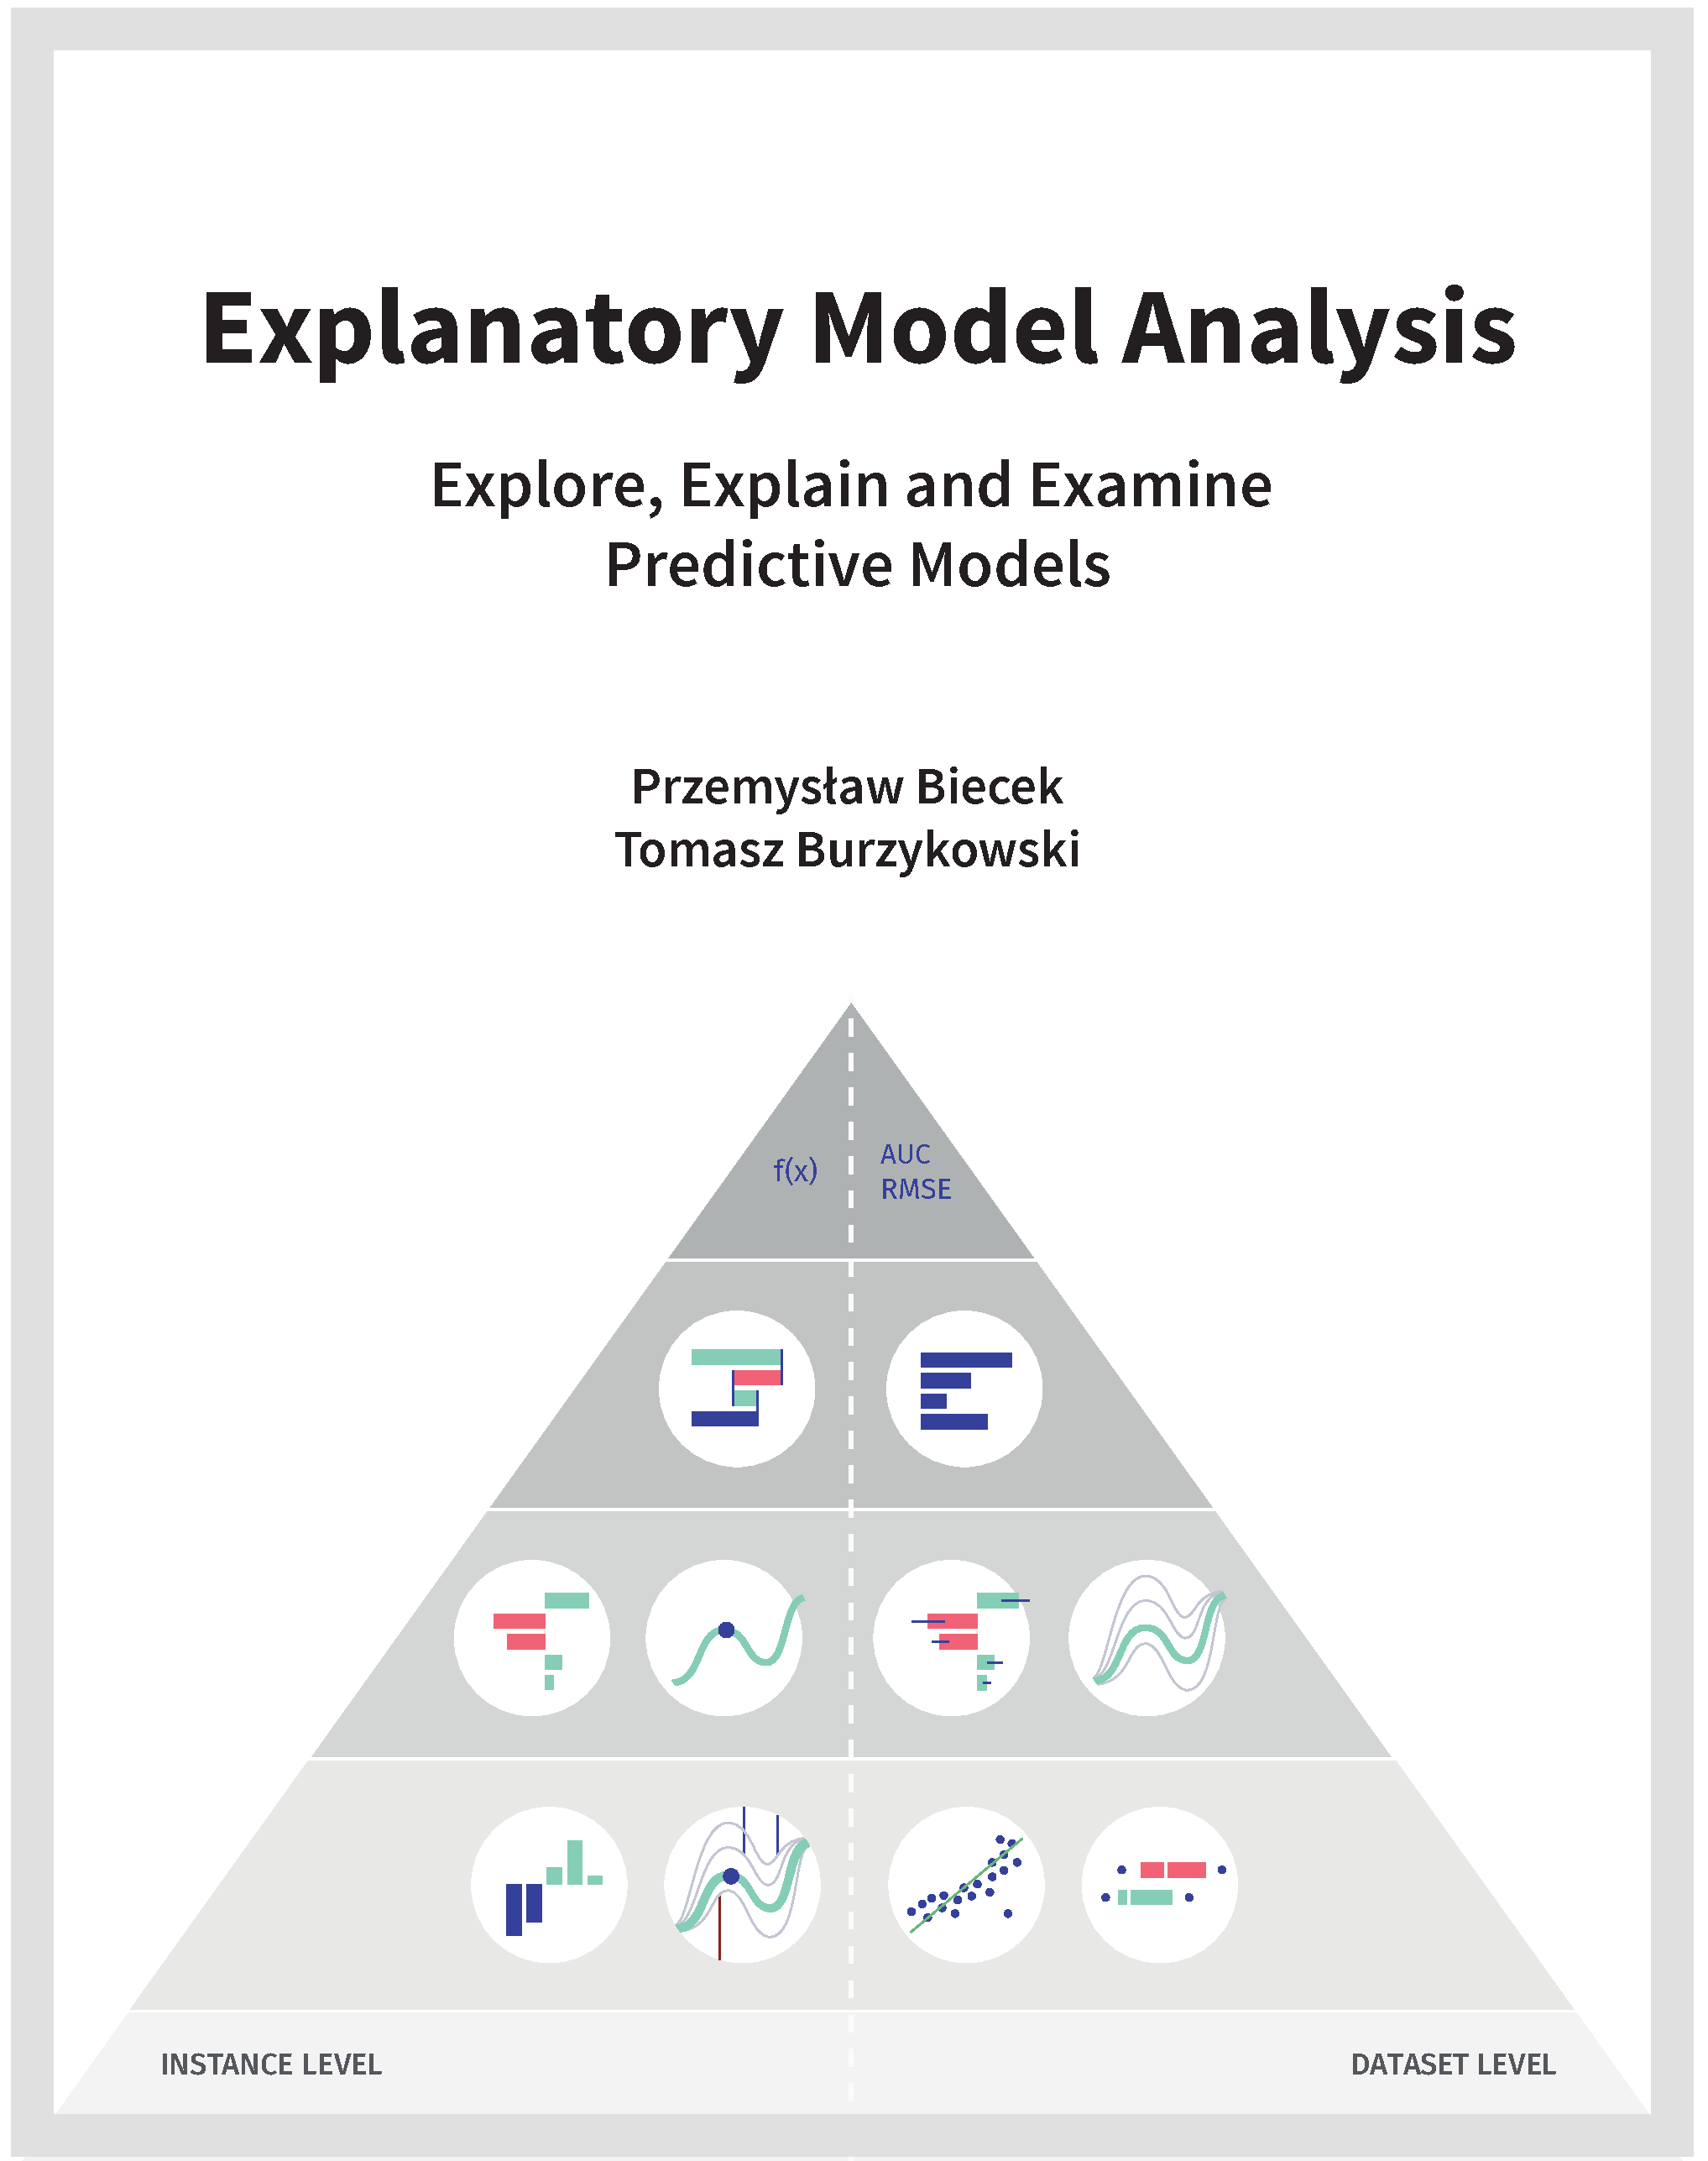
\includegraphics[width=0.99\linewidth]{figure/front4} \end{center}

\hypertarget{why-explore}{%
\section*{Why explore}\label{why-explore}}
\addcontentsline{toc}{section}{Why explore}

\hypertarget{introduction}{%
\section{Introduction}\label{introduction}}

\hypertarget{notes-to-readers}{%
\subsection{Notes to readers}\label{notes-to-readers}}

A note to readers: this text is a work in progress.

We've released this initial version to get more feedback. Feedback can be given at the GitHub repo \url{https://github.com/pbiecek/ema/issues}. We are primarily interested in the organization and consistency of the content, but any comments will be welcomed.

We'd like to thank everyone that contributed feedback, found typos, or ignited discussions while the book was being written, including GitHub contributors: \href{https://github.com/agosiewska/}{agosiewska}, Rees Morrison, \href{https://github.com/kasiapekala/}{kasiapekala}, \href{https://github.com/hbaniecki/}{hbaniecki}, \href{https://github.com/AsiaHenzel/}{AsiaHenzel}, \href{https://github.com/kozaka93/}{kozaka93},
\href{https://github.com/agilebean/}{agilebean}.

\hypertarget{the-aim-of-the-book}{%
\subsection{The aim of the book}\label{the-aim-of-the-book}}

Predictive models are used to guess (statisticians would say: predict) values of a variable of interest based on other variables. As an example, consider prediction of sales based on historical data, prediction of risk of heart disease based on patient characteristics, or prediction of political attitudes based on Facebook comments.

Predictive models have been constructed through the entire human history. Ancient Egyptians, for instance, used observations of the rising of Sirius to predict flooding of the Nile. A more rigorous approach to model construction may be attributed to the method of least squares, published more than two centuries ago by Legendre in 1805 and by Gauss in 1809. With time, the number of applications in economy, medicine, biology, and agriculture has grown. The term \emph{regression} was coined by Francis Galton in 1886. Initially, it was referring to biological applications, while today it is used for various models that allow prediction of continuous variables. Prediction of nominal variables is called \emph{classification}, and its beginning may be attributed to works of Ronald Fisher in 1936.

During the last century, many statistical models that can be used for predictive purposes have been developed. These include linear models, generalized linear models, regression and classification trees, rule-based models, and many others. Developments in mathematical foundations of predictive models were boosted by increasing computational power of personal computers and availability of large datasets in the era of ,,big data'\,' that we have entered.

With the increasing demand for predictive models, model features such as flexibility, ability to perform internally variable selection (feature engineering), and high precision of predictions are of interest. To obtain robust models, ensembles of models are used. Techniques like bagging, boosting, or model stacking combine hundreds or thousands of small models into a one super-model. Large deep neural models have over a billion parameters.

There is a cost of this progress. Complex models may seem to operate like ,,black boxes'`. It may be difficult, or even impossible, to understand how thousands of coefficients affect the model prediction. At the same time, complex models may not work as well as we would like them to. An overview of real problems with massive-scale black-box models may be found in an excellent book of Cathy O'Neil \citep{ONeil} or in her TED Talk ,,\emph{The era of blind faith in big data must end}''. There is a growing number of examples of predictive models with performance that deteriorated over time or became biased in some sense. For instance, IBM's Watson for Oncology was criticized by oncologists for delivering unsafe and inaccurate recommendations \citep{IBMWatson}. Amazon's system for CV screening was found to be biased against women \citep{AmazonAI}. The COMPAS (Correctional Offender Management Profiling for Alternative Sanctions) algorithm for predicting recidivism, developed by Northpointe (now Equivant), is accused to be biased against blacks \citep{COMPAS}. Algorithms beyond Apple Credit Card are accused to be gender-biased \citep{AppleCreditCard}. Some tools for sentiment analysis are suspected to be age-biased \citep{Diaz2018}. These are examples of models and algorithms that led to serious violations of fairness and ethical principles. An example of situation when data drift led to deterioration in model performance is the Google Flu model, which gave worse predictions after two years than at baseline \citep{GoogleFLU}, \citep{Lazer1203}.

A reaction to some of these examples and problems are new regulations, like the General Data Protection Regulation \citep{EUGDPR}. Also, new civic rights are being formulated \citep{RightToExpl}, \citep{RightToExpl2}, \citep{RightToExpl3}. A noteworthy example is the \emph{,,Right to Explanation'\,'}, i.e., the right to be provided an explanation for an output of an automated algorithm \citep{RightToExpl}. To exercise the right, we need new methods for verification, exploration, and explanation of predictive models.

Figure \ref{fig:UMEPImportance} shows how the increase in the model complexity affects the relative importance of domain understanding vs.~modeling vs.~validation. Simplest models are usually built on top of a good understanding of the domain. Domain knowledge helps to create and select most important variables that can be transformed into predictive scores. Machine learning exploits the tradeoff between availability of data and domain knowledge. Flexible models can use massive data to learn good features and filter out bad ones. The effort is shifted from a deep understanding of the domain towards computationally heavy training of models. The validation part is of an increased importance because it creates a feedback loop with the modeling. Results from model validation lead to next decisions related to model training. This is different than in case of statistical hypothesis testing. Statistical hypotheses shall be stated in advance of data analysis and obtained p-values shall not interfere in the way how data or models were prepared.

What will be next? The increasing automation in the EDA (Exploratory Data Analysis) and modeling part of the process shift the focus towards the validation of models. The purpose of validation is not only to measure how good is the model but also what other risks are associated with models. Risks like concept drift, gender, age or race bias. This book is about new methods that can be used for validation and justification.

\begin{figure}

{\centering \includegraphics[width=0.9\linewidth]{figure/UMEPImportance} 

}

\caption{Shift in the relative importance and effort put in different phases of the data-driven modeling. (A) Statistical modeling is often based on deep understanding of the domain. Manual data exploration, consultations with domain experts, variable transformations lead to good models. Structures of models are often based on (generalized) linear models. Model verification is done through hypothesis testing. (B) Machine learning modeling is often based on elastic models fitted to large volumes of data. Domain exploration is often shallow while the focus is based on predictive performance. Lots of attention is put in cross validation and other strategies that deal with overfitting. (C) What will be next? Human-centered modeling? Better tools for auto EDA and auto ML will shift focus into the part related with validation against the domain knowledge like fairness, bias or new techniques for data exploration. Arrows show feedback loops in the modeling process. The feedback loop is even larger now, as the results from model validation are helping also in the domain understanding.}\label{fig:UMEPImportance}
\end{figure}

Out of this we can conclude that, today, the true bottleneck in predictive modelling is not the lack of data, nor the lack of computational power, nor inadequate algorithms, nor the lack of flexible models. It is the lack of tools for model validation, model exploration, and explanation of model decisions. Thus, in this book, we present a collection of methods that may be used for this purpose. As development of such methods is a very active area of research and new methods become available almost on a continuous basis, we do not aim at being exhaustive. Rather, we present the mind-set, key problems, and several examples of methods that can be used in model exploration.

\hypertarget{three-single-laws}{%
\subsection{A bit of philosophy: three laws of model explanation}\label{three-single-laws}}

In 1942, Isaac Asimov forumlated \href{https://en.wikipedia.org/wiki/Three_Laws_of_Robotics}{Three Laws of Robotics}:

\begin{enumerate}
\def\labelenumi{\arabic{enumi})}
\tightlist
\item
  a robot may not injure a human being,
\item
  a robot must obey the orders given it by human beings, and
\item
  a robot must protect its own existence.
\end{enumerate}

Today's robots, like cleaning robots, robotic pets, or autonomous cars are far from being conscious enough to fall under Asimov's ethics. However, we are more and more surrounded by complex predictive models and algorithms used for decision making. Artificial Intelligence models are used in health care, politics, education, justice, and many other areas. The models and algorithms have a far larger influence on our lives than physical robots. Yet, applications of such models are left unregulated despite examples of their potential harmfulness. See \emph{Weapons of Math Destruction} by Cathy O'Neil \citep{ONeil} for an excellent overview of selected problems.

It's clear that we need to control the models and algorithms that may affect us. Thus, Asimov's laws are referred to in the context of the discussion around \href{https://en.wikipedia.org/wiki/Ethics_of_artificial_intelligence}{Ethics of Artificial Intelligence}. Initiatives to formulate principles for AI development have been undertaken, for instance, in the UK {[}Olhede \& Wolfe, Significance 2018, 15: 6-7{]}. Following Asimov's approach, we propose three requirements that any predictive model should fulfill:

\begin{itemize}
\tightlist
\item
  \textbf{Prediction's validation}. For every prediction of a model, one should be able to verify how strong is the evidence that confirms the prediction.
\item
  \textbf{Prediction's justification}. For every prediction of a model, one should be able to understand which variables affect the prediction and to what extent.
\item
  \textbf{Prediction's speculation}. For every prediction of a model, one should be able to understand how the model prediction would change if input variables changed.
\end{itemize}

We see two ways to comply with these requirements. One is to use only models that fulfill these conditions by design. There are so called interpretable by design models like linear models, rule based models or classification trees with small number of parameters \citep{molnar2019}. However, the price for transparency may be a reduction in performance. Another way is to use tools that allow, perhaps by using approximations or simplifications, to ,,explain'\,' predictions for any model. In our book, we will focus on the latter approach.

\hypertarget{bookstructure}{%
\subsection{The structure of this book}\label{bookstructure}}

This book is split in two major parts. In the part \emph{Instance-level explainers}, we present techniques for exploration and explanation of model predictions for a single observation. On the other hand, in the part \emph{Dataset-level explainers}, we present techniques for exploration and explanation of a model for an entire dataset.

Before embarking on the description of the methods, in Chapter
\ref{modelDevelopmentProcess}, we provide a short introduction to the process of data exploration and model assembly along with notation and definition of key concepts that are used in consecutive chapters.
In chapters \ref{doItYourselfWithR} and \ref{doItYourselfWithPython}, we provide a short description of R and Python tools and packages that are necessary to replicate the results presented in this book. In Chapter \ref{dataSetsIntro}, we describe two datasets that are used throughout the book to illustrate the presented methods and tools.



\begin{figure}

{\centering 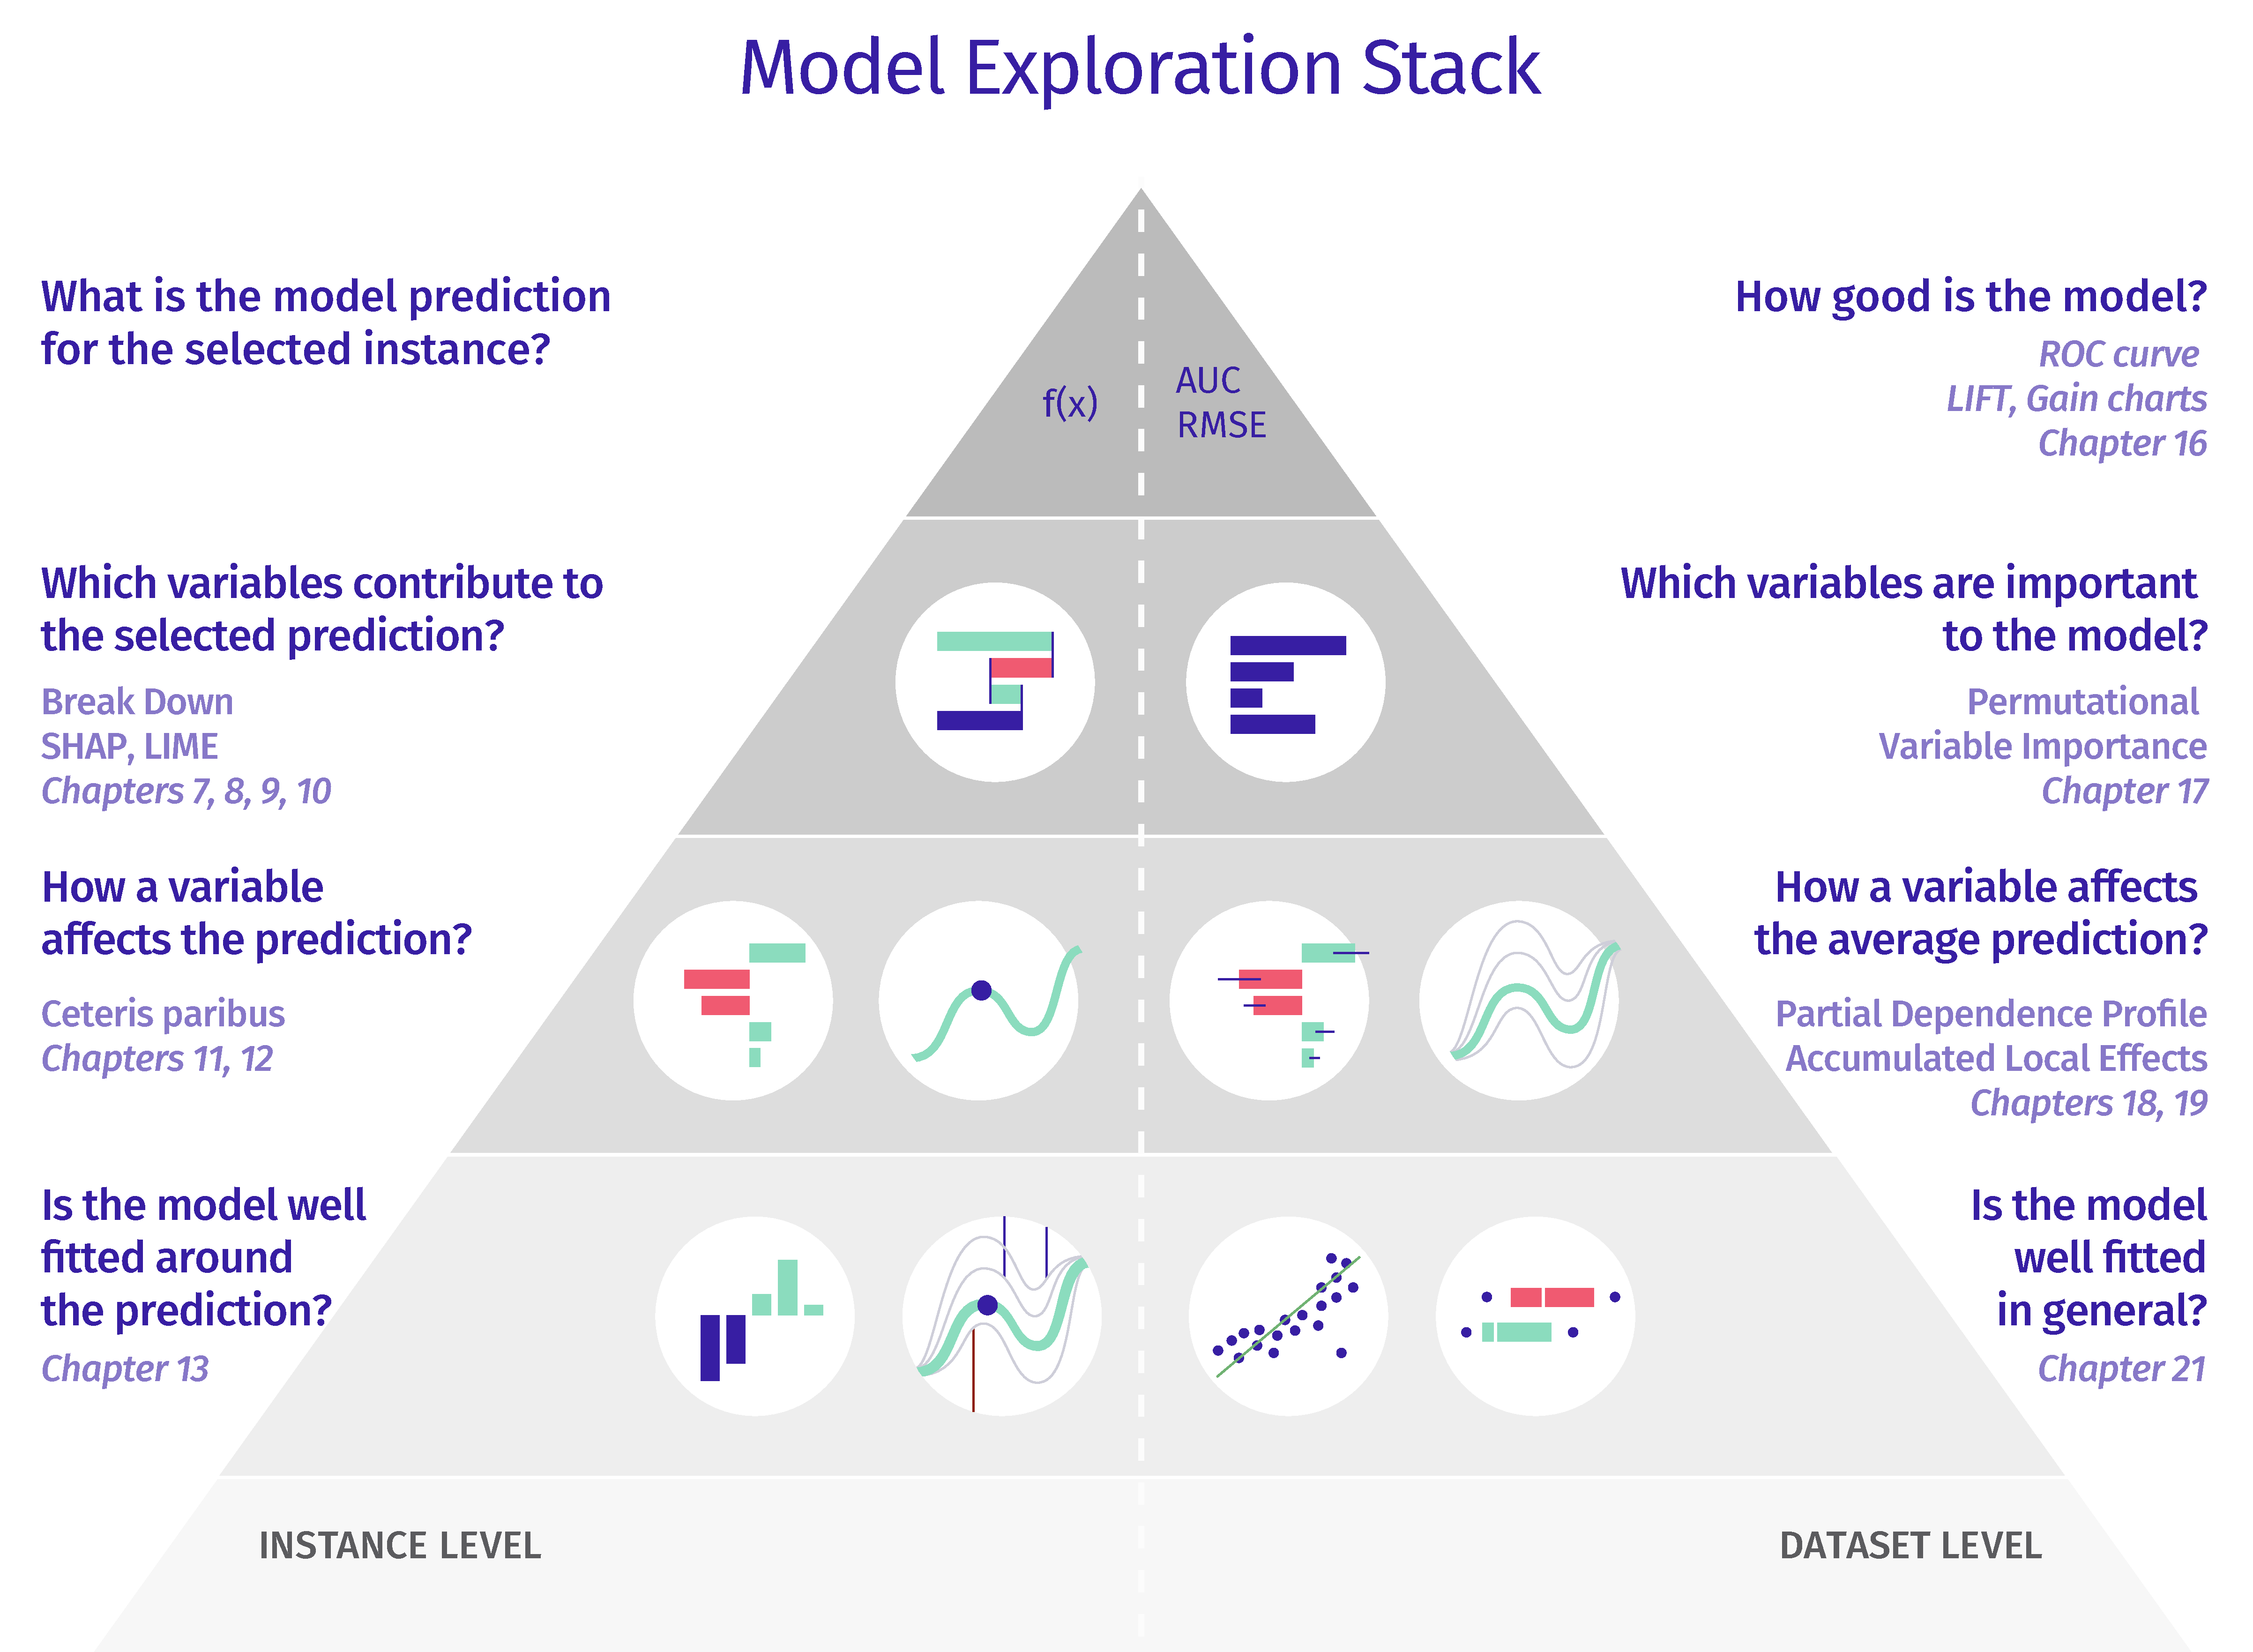
\includegraphics[width=0.85\linewidth]{figure/UMEPpiramide} 

}

\caption{Stack with model exploration methods presented in this book. Left side is focused on instance-level explanation while the right side is focused on dataset-level explanation. Consecutive layers of the stack are linked with a deeper level of model exploration. These layers are linked with law's of model exploration introduced in Section \ref{three-single-laws}}\label{fig:UMEPpiramide}
\end{figure}

Rest of the book is structured in Figure \ref{fig:UMEPpiramide}.

The \textbf{Instance-level} part of the book consists of Chapters \ref{breakDown}-\ref{summaryInstanceLevel}.
Chapters \ref{breakDown}-\ref{shapley} present methods to decompose model predictions into variable contributions. In particular, Chapter \ref{breakDown} introduces Break-down (BD) plots for models with additive effects. On the other hand, Chapter \ref{iBreakDown} presents a method that allows for interactions. Finally, Chapter \ref{shapley} describes SHAP \citep{SHAP} an alternative method for decomposing model predictions that is closely linked with Shapley values \citep{shapleybook1952} developed originally for cooperative games.
Chapter \ref{LIME} presents a different approach to explanation of single-instance predictions. It is based on a local approximation of a black-box model by a simpler, glass-box one. In this chapter, we discuss the Local Interpretable Model-Agnostic Explanations (LIME) method \citep{lime}. These chapters corresponds to the second layer of the stack in Figure \ref{fig:UMEPpiramide}.

In Chapters \ref{ceterisParibus}-\ref{localDiagnostics} we present methods based on Ceteris-paribus (CP) profiles. The profiles show the change of model-based predictions induced by a change of a single variable. These profiles are introduced in Chapter \ref{ceterisParibus} while Chapter \ref{ceterisParibusOscillations} presents a CP-profile-based measure that summarizes the impact of a selected variable on model's predictions. This measure can be used to determine the order of variables in model exploration. It is particularly important for models with large numbers of explanatory variables. Chapter \ref{localDiagnostics} is focused on model diagnostic. It describes local-fidelity plots that are useful to investigate the sources of a poor prediction for a particular single observation.
The final chapter of the first part, Chapter \ref{summaryInstanceLevel} compares various instance-level explainers.

The \textbf{Dataset-level explainers} part of the book consists of Chapters \ref{modelLevelExploration}-\ref{residualDiagnostic}. These chapters present methods in the same order as appeared in the Model Exploration Stack in Figure \ref{fig:UMEPpiramide}.
Chapter \ref{modelPerformance} shows selected measures for model benchmarking along with performance measures for classification and regression models.
On top of these measures, the Chapter \ref{featureImportance} presented an algorithm for assessment of importance of variables based on selected performance measure. This method is model agnostic and can be used for cross models comparisons.
Next layer of the Model Exploration Stack is presented in Chapters \ref{partialDependenceProfiles} and \ref{accumulatedLocalProfiles}. Here we introduce Partial Dependency and Accumulated Dependency methods for univariate exploration of variable effects.
This part of the book is closed with the Chapter \ref{residualDiagnostic} that summarises diagnostic techniques for model residuals.

To make the exploration of the book easier, in each Chapter we introduce a single method and each chapter has the same structure:

\begin{itemize}
\tightlist
\item
  Section \emph{Introduction} explains the goal of and the general idea behind the method.
\item
  Section \emph{Method} shows mathematical or computational details related to the method. This subsection can be skipped if you are not interested in the details.
\item
  Section \emph{Example} shows an exemplary application of the method with discussion of results.
\item
  Section \emph{Pros and cons} summarizes the advantages and disadvantages of the method. It also provides some guidance regarding when to use the method.
\item
  Section \emph{Code snippets} shows the implementation of the method in R and Python. This subsection can be skipped if you are not interested in the implementation.
\end{itemize}

\hypertarget{terminology}{%
\subsection{Terminology}\label{terminology}}

It is worth noting that, when it comes to predictive models, the same concepts have often been given different names in statistics and in machine learning. For instance, in the statistical-modelling literature, one refers to ,,explanatory variables,'\,' with ,,independent variables,'\,' ,,predictors,'\,' or ,,covariates'\,' as often-used equivalents. Explanatory variables are used in the model as means to explain (predict) the ,,dependent variable,'\,' also called ,,predicted'\,' variable or ,,response.'\,' In machine-learning terminology, ,,input variables'\,' or ,,features'\,' are used to predict the ,,output'\,' or ,,target'\,' variable. In statistical modelling, models are fit to the data that contain ,,observations'`, whereas in the machine-learning world a dataset may contain ,,instances'' or ,,cases'`. When we talk about values that define a single instance of a model in statistical modelling we refer to model ,,coefficients'' while in machine-learning it is more common to use phrase model ,,parameters'`. In statistics it is common to say that model coefficients are ,,estimated'' while in machine learning it is more common to say that parameters are ,,trained'\,' or are obtained in the process of ,,model training'\,'.

To the extent possible, in our book we try to consistently use the statistical-modelling terminology. However, the reader may find references to a ,,feature'\,' here and there. Somewhat inconsistently, we also introduce the term ,,instance-level'\,' explanation. Instance-level explanation methods are designed to extract information about the behavior of the model related to a specific observation (or instance). On the other hand, ,,dataset-level'\,' explanation techniques allow obtaining information about the behavior of the model for an entire dataset.

We consider models for dependent variables that can be continuous or nominal/categorical. The values of a continuous variable can be represented by numbers with an ordering that makes some sense (zip codes or phone numbers are not considered as continuous variables while age, number of children are). A continuous variable does not have to be continuous in the mathematical sense; counts (number of floors, steps, etc.) will be treated as continuous variables as well. A nominal/categorical variable can assume only a finite set of values that are not numbers in the mathematical sense, i.e.~it makes no sense to subtract or divide these values.

In this book we focus on ,,black-box'\,' approach. We discuss this approach in a bit more detail in the next section.

\hypertarget{glass-box-models-vs.-black-box-models}{%
\subsection{Glass-box models vs.~black-box models}\label{glass-box-models-vs.-black-box-models}}

Black-box models are models with a complex structure that is hard to understand by humans. Usually this refers to a large number of model coefficients or complex mathematical transformations. As people vary in their capacity to understand complex models, there is no strict threshold for the number of coefficients that makes a model a black-box. In practice, for most people this threshold is probably closer to 10 than to 100.

A ,,glass-box'\,' (sometimes called white-box or transparent-box) model, which is opposite to a ,,black-box'\,' one, is a model that is easy to understand (though maybe not by every person). It has a simple structure and a limited number of coefficients.

The most common classes of glass-box models are decision or regression trees, as an example in Figure \ref{fig:BILLCD8}, rules, or models with an explicit compact structure, like the following model for obesity based on the BMI index.

\[
BMI = \frac{mass_{kg}}{height_{m^2}}.
\]

In the model, two explanatory variables are used, mass in kilograms and height in meters. Based on them a BMI index is derived that commonly used for classification into \emph{Underweight} (BMI \textless{} 18), \emph{Normal} (18 \textless{} BMI \textless{} 25) or \emph{Overweight} (BMI \textgreater{} 25) categories. Having the model in a compact form it is easy to understand how changes in one variable affect the model output.

The structure of a glass-box model is, in general, easy to understand. It may be difficult to collect the necessary data, build the model, fit it to the data, or perform model validation, but once the model has been developed its interpretation and mode of working is straightforward.

Why is it important to understand the model structure? There are several important advantages. If the model structure is clear, we can easily see which variables are included in the model and which are not. Hence, for instance, we may be able to, question the model when a particular explanatory variable was excluded from it. Also, in the case of a model with a clear structure and a limited number of coefficients, we can easily link changes in model predictions with changes in particular explanatory variables. This, in turn, may allow us to challenge the model against domain knowledge if, for instance, the effect of a particular variable on predictions is inconsistent with previously established results. Note that linking changes in model predictions with changes in particular explanatory variables may be difficult when there are many variables and/or coefficients in the model. For instance, a classification tree with hundreds of nodes is difficult to understand, as is a linear regression model with hundreds of coefficients.

\begin{figure}

{\centering \includegraphics[width=0.5\linewidth]{figure/wbBILL8model} 

}

\caption{Example classification tree model for melanoma risk patients based on [@BILLCD8]. The model is based on two explanatory variables, Breslow thickness and Tumor infiltration lymphocytes. These two variables lead to three groups of paritents with different odds of survival.}\label{fig:BILLCD8}
\end{figure}

Note that some glass-box models, like the decision tree model presented in Figure \ref{fig:BILLCD8} by design satisfies explainability laws introduced in Section \ref{three-single-laws}.
For \emph{Prediction's validation} we see in each node how many patients fall in a given category. For \emph{Prediction's justification} we see which variables are used in every decision path. For \emph{Prediction's speculation} we can trace how changes in particular variables will affect the model prediction. We can, of course, argue if the model is good or not, but obviously the model structure is transparent.

Comprehending the performance of a black-box models presents more challenges. The structure of a complex model, such as a neural-network model, may be far from transparent. Consequently, we may not understand which features influence the model decisions and by how much. Consequently, it may be difficult to decide whether the model is consistent with our domain knowledge. In our book we present tools that can help in extracting the information necessary for the evaluation of complex models.

\hypertarget{model-agnostic-vs.-model-specific-approach}{%
\subsection{Model-agnostic vs.~model-specific approach}\label{model-agnostic-vs.-model-specific-approach}}

Interest in model interpretability is as old as the statistical modeling itself.
Some classes of models have been developed for a long period of time or have attracted intensive research. Consequently, those classes of models are equipped with excellent tools for model exploration or visualisation. For example:

\begin{itemize}
\tightlist
\item
  There are many tools for diagnostics and evaluation of linear models, see for example \citep{Galecki2013} or \citep{Faraway02practicalregression}. Model assumptions are formally defined (normality, linear structure, homogenous variance) and can be checked by using normality tests or plots (normal qq-plot), diagnostic plots, tests for model structure, tools for identification of outliers, etc.
\item
  For many more advanced models with an additive structure, like the proportional hazards model, many tools can be used for checking model assumptions, see for example \citep{rms} or \citep{sheather2009modern}.
\item
  Random-forest models are equipped with the out-of-bag method of evaluating performance and several tools for measuring variable importance \citep{R-randomForest}. Methods have been developed to extract information from the model structure about possible interactions \citep{randomForestExplainer}. Similar tools have been developed for other ensembles of trees, like boosting models (xgboost, gbm). See \citep{xgboostExplainer} or \citep{EIXkarbowiak}.
\item
  Neural networks enjoy a large collection of dedicated model-explanation tools that use, for instance, the layer-wise relevance propagation technique \citep{BachLWRP}, or saliency maps technique \citep{SaliencyMaps}, or a mixed approach. Broader summary is presented in \citep{samek2017explainable} and \citep{alber2018innvestigate}.
\item
  BERT family of models leads to high-performance models in Natural Language Processing. The exBERT method \citep{hoover2019exbert} is designed to visualize the activation of attention heads in this model.
\end{itemize}

Of course, the list of model classes with dedicated collections of model-explanation and/or diagnostics methods is much longer. This variety of model-specific approaches does lead to issues, though. For instance, one cannot easily compare explanations for two models with different structures. Also, every time a new architecture or a new ensemble of models is proposed, one needs to look for new methods of model exploration. Finally, for brand-new models no tools for model explanation or diagnostics may be immediately available.

For these reasons, in our book we focus on model-agnostic techniques. In particular, we prefer not to assume anything about the model structure, as we may be dealing with a black-box model with an unspecified structure. Often we do not have access to model parameters just to a specified Application Programming Interface (API) that allows for querying remote models (for example in Microsoft Cognitive Services \citep{MicrosofrCognitiveServices}).
In that case, the only operation that we may be able to perform is the evaluation of a model for a specified data.

However, while we do not assume anything about the structure of the model, we will assume that the model operates on \(p\)-dimensional vector of variables/features and, for a single observation, it returns a single value (score/probability) which is a real number. This assumption holds for a broad range of models for data such as tabular data, images, text data, videos, etc. It may not be suitable for, e.g., models with memory like sequence-to-sequence models \citep{seq2seq} or Long Short Term Memory models \citep{lstm} in which the model output depends also on sequence of previous inputs or generative models that output text of images.

\hypertarget{what-is-in-this-book-and-what-is-not}{%
\subsection{What is in this book and what is not}\label{what-is-in-this-book-and-what-is-not}}

The area of model exploration and explainability is quickly growing and is present in many different flavors. Instead of showing every existing method (is it really possible?) we rather selected a subset of consistent tools that are a good starting set for model exploration. Our focus was on the impact of the model exploration and explanation tools rather than on selected methods. We believe that once we become aware of potential beyond visual model exploration, once we will learn a language of model explanation, we will improve our process of data modeling.

Taking this goal into account \textbf{in this book, we do show}

\begin{itemize}
\tightlist
\item
  how to determine features that affect model prediction for a single observation. In particular, we present the theory and examples of methods that can be used to explain prediction like Break Down plots, Ceteris Paribus profiles, local-model approximations, or Shapley values;
\item
  techniques to examine fully-trained machine-learning models as a whole. In particular, we review the theory and examples of methods that can be used to explain model performance globally, like partial-dependence plots, variable-importance plots, and others;
\item
  charts that can be used to present key information in a quick way;
\item
  tools and methods for model comparison;
\item
  code snippets for R and Python that explain how to use the described methods.
\end{itemize}

On the other hand, \textbf{in this book, we do not focus on}

\begin{itemize}
\tightlist
\item
  any specific model. The techniques presented are model agnostic and do not make any assumptions related to the model structure;
\item
  data exploration. There are very good books on this topic, like \emph{R for Data Science} by Garrett Grolemund and Hadley Wickham \citep{r4ds2019} or \emph{Python for Data Analysis} \citep{Wes2012} by Wes McKinney or an excellent \emph{Exploratory Data Analysis} by John Tukey \citep{tukey1977};
\item
  the process of model building. There are also very good books on this topic, see \emph{Modern Applied Statistics with S} by W. Venables and B. Ripley \citep{MASSbook}, \emph{An Introduction to Statistical Learning} by Gareth James, Daniela Witten, Trevor Hastie and Robert Tibshirani \citep{James20147} or \emph{Computer Age Statistical Inference} by Bradley Efron and Trevor Hastie \citep{Efron2016};
\item
  any particular tools for model building. These are discussed, for instance, in \emph{Applied Predictive Modeling} by Max Kuhn and Kjell Johnson \citep{Kuhn2013}.
\end{itemize}

\hypertarget{thanksto}{%
\subsection{Acknowledgements}\label{thanksto}}

This book has been prepared using the \texttt{bookdown} package \citep{R-bookdown}, created thanks to the amazing work of Yihui Xie.
Figures and tables are created in R language for statistical computing \citep{RcoreT} with numerous libraries that support predictive modeling. Just to name few frequently used in this book \texttt{randomForest} \citep{randomForest}, \texttt{ranger} \citep{rangerRpackage}, \texttt{rms} \citep{rms}, \texttt{gbm} \citep{gbm} or \texttt{caret} \citep{caret}. For statistical graphics we used the \texttt{ggplot2} library \citep{ggplot2} and for model governance we used \texttt{archivist} \citep{archivist}.

Przemek's work on interpretability started during research trips within the RENOIR (H2020 grant no. 691152) secondments to Nanyang Technological University (Singapour) and Davis University of California (USA). So he would like to thank Prof.~Janusz Holyst for the chance to take part in this project. Przemek would also like to thank Prof.~Chris Drake for her hospitality. This book would have never been created without perfect conditions that Przemek found at Chris's house in Woodland.

\hypertarget{modelDevelopmentProcess}{%
\section{Model Development}\label{modelDevelopmentProcess}}

\hypertarget{MDPIntro}{%
\subsection{Introduction}\label{MDPIntro}}

In this book we present methods that can be used for exploration and explanation of predictive models. But before we can explore a model, first we need to train one.

In this part of the book we overview the process of model development and introduce steps that lead to a model creation. It is not a comprehensive manual ,,how to train a model in 5 steps'\,'. The goal of this chapter is to show what needs to be performed before we can do any diagnostic or exploration of a trained model.

Predictive models are created for different purposes. Sometimes it is a team of data scientists that spend months on a single model that will be used for model scoring in a big financial company. Every detail is important for models that operate on large scale and have long-term consequences. Another time it is an in-house model trained for prediction of a demand for pizza. The model is developed by a single person in few hours. If model will not perform well it will be updated, replaced or removed.

Whatever it is a large model or small one, similar steps are to be taken during model development.

\hypertarget{MDPprocess}{%
\subsection{The Process}\label{MDPprocess}}

Several approaches are proposed in order to describe the process of model development. Their main goal is to standardize the process. And the standardisation is important because it helps to plan resources needed to develop and maintain the model and also to not miss any important step.

The most known methodology for data science projects is CRISP-DM \citep{crisp1999}, \citep{crisp2019wiki} which is a tool agnostic procedure. The key component of CRISP-DM is the break down of the whole process into six phases, that are iterated: business understanding, data understanding, data preparation, modeling, evaluation and deployment. CRISP-DM is general, it was designed for any data science project. For predictive models some methodologies are introduced in \citep{r4ds2019} and \citep{misconceptions2019}.Both are focused on iterative repetitions of some phases.
Figure \ref{fig:MDPwashmachine} presents a variant of iterative process divided into five steps. Data preparation is needed prior to any modeling. Better data is needed for better models. On the other hand, garbage-in garbage-out. Once the data is gathered, steps that are usually highlighted are Data understanding, Model assembly and Model audit. This is the common thinking about model development. Repeat these steps until some convergence, e.g.~repeat until best model is identified.

\begin{figure}

{\centering \includegraphics[width=0.6\linewidth]{figure/MDP_washmachine} 

}

\caption{Lifecycle of predictive model can be decomposed into five tasks. First we need data that is poured into the model development cycle. The model development is highly iterative, learn something new about the data, assemble a new model based on current understanding, and validate the new model. Repeat these steps as long as needed to be satisfied with model performance. Once the model is created we can deliver the model to the production along with required tests and documentation.}\label{fig:MDPwashmachine}
\end{figure}

In this book we use \emph{Model Development Process} introduced in \citep{mdp2019}. It is motivated by Rational Unified Process for Software Development \citep{rup1998}, \citep{usdp1999}, \citep{spiral1988}. One can think about MDP as an extension of process introduced in Figure \ref{fig:MDPwashmachine}. What is important is to notice that consecutive iterations are not identical. Our knowledge increases during the process and consecutive iterations are performed with different goals in mind.

This is why MDP is build as an untangled version of Figure \ref{fig:MDPwashmachine}. The MDP process is shown in Figure \ref{fig:mdpGeneral}. Each vertical stripe is a single run of the cycle.
First iterations are usually focused on \emph{formulation of the problem}. Sometimes the problem is well stated, however it's a rare situation valid maybe only for kaggle competitions. In most real-life problems the problem formulation requires lots of discussions and experiments. Once the problem is defined we can start building first prototypes, first \emph{crisp versions of models}. These initial versions of models are needed to verify if the problem can be solved and how far we are form the solution. Usually we gather more information and go for the next phase, the \emph{fine tuning}. We repeat these iterations until a final version of a model is developed. Then we move to the last phase \emph{maintenance and} (one day) \emph{decommissioning}.



\begin{figure}

{\centering \includegraphics[width=0.99\linewidth]{figure/mdp_general} 

}

\caption{Overview of the Model Development Process. Horizontal axis show how time passes from the problem formulation to the model decommissioning. Vertical axis shows tasks are performed in a given phase. Each vertical strip is a next iteration of cycle presented in Figure \ref{fig:MDPwashmachine}}\label{fig:mdpGeneral}
\end{figure}

Having in mind the map of model development we can point places where one can use methods presented in this book.

As suggested in the title of this book, three primary applications are: exploration, explanation and debugging. \emph{Exploration} refers to situations in which we better understand the data and the domain. Presented techniques can be used to speed up the variable engineering or variable selection. \emph{Explanation} refers to situations in which we are interested in decision paths beyond particular predictions. \emph{Debugging} refers to situations in which we want to understand weak points of a model and correct them. These applications target phases Data understanding, Model assembly and Model audit.

In this book we present various examples based on three use cases. Two introduced in Chapter \ref{dataSetsIntro} (binary classification in surviving Titanic sinking and regression in apartments pricing) and one in Chapter \ref{UseCaseFIFA} (estimation of soccer player value based on its skills). Due to space limitation we do not show the full life cycle of these problems, but we are focused on phases Crisp modeling and Fine tuning.

Rest of this chapter is focused on a brief overview of the notation and commonly used methods for data exploration, model training and model validation.

\hypertarget{notation}{%
\subsection{Notation}\label{notation}}

Methods described in this book were developed by different authors, who used different mathematical notations.
We try to keep the mathematical notation consistent throughout the entire book. In some cases this may result in formulas with a fairly complex system of indices.

In this section, we provide a general overview of the notation we use. Whenever necessary, parts of the notation will be explained again in subsequent chapters.

We assume that the data consist \(n\) observations/instances. Each observation is described by \(p\) explanatory variables. Thus data is described as a set of points on a \textbf{\(p\)-dimensional input space} \(\mathcal X \equiv \mathcal R^p\). By \(x \in \mathcal X\) we will refer to a single point in this input space.
By \(x_i\) we refer to the \(i\)-th observation in this dataset. Of course, \(x_i \in \mathcal X\). By \(X\) we denote a matrix \(n\times p\) with rows corresponding to consecutive observations.

Some methods of model exploration are constructed around an observation of interest which will be denoted by \(x_{*}\). The observation may not necessarily belong to the analyzed dataset; hence, the use of the asterisk in the index. Of course, \(x_* \in \mathcal X\).

Points in \(\mathcal X\) are \(p\) dimensional vectors. We refer to the \(j\)-th coordinate by using \(j\) in superscript. Thus, \(x^j_i\) denotes the \(j\)-th coordinate of the \(i\)-th observation from the analyzed dataset. If \(\mathcal J\) denotes a subset of indices, then \(x^{\mathcal J}\) denotes the elements of vector \(x\) corresponding to the indices included in \(\mathcal J\).

We will use the notation \(x^{-j}\) to refer to a vector that results from removing the \(j\)-th coordinate from vector \(x\). By \textbf{\(x^{j|=z}\)}, we denote a vector with the values at all coordinates equal to the values in \(x\), except of the \(j\)-th coordinate, which is set equal to \(z\). So, if \(w=x^{j|=z}\), then \(w^j = z\) and \(\forall_{k\neq j} w^k = x^k\). In other words \(x^{j|=z} = (x^1, ..., x^{j-1}, z, x^{j+1}, ..., x^p)\).

By \(x^{*j}\) we denote a matrix with the values as in \(x\) except the \(j\)th column which is permuted.

In this book, a model is a function \(f:\mathcal X \rightarrow \mathcal R\) that transforms a point from \(\mathcal X\) into a real number. In most cases, the presented methods can be used directly for multivariate dependent variables; however, we use examples with uni-variate responses to simplify the notation.
Typically, during the model development, we create many competing models. Formally we shall index models to refer to a specific version of a trained model. But for the sake of simplicity we omit these indexes where they are not important.

Later in this book we will use the term \textbf{model residual} as the the difference between the observed value of the dependent variable \(Y\) for the \(i\)-th observation from a particular dataset and the model prediction for the observation

\begin{equation}
r_i = y_i - f(x_i) = y_i - \hat y_i.
\label{eq:modelResiduals}
\end{equation}

\hypertarget{data-exploration}{%
\subsection{Data exploration}\label{data-exploration}}

Before we start the modeling we need to understand the data.
Visual, tabular and statistical tools for data exploration are used depending on the character of variables.

The most know introduction to data exploration is the famous book by John Tukey \citep{tukey1977}. It introduces new tools for data exploration, like for example boxplots or stem-and-leaf plots. Availability of computational tools makes the process of data exploration easier and more interactive. Find a good overview of techniques for data exploration in \citep{Nolan2015} or \citep{Wickham2017}.

In this book we will rely on five visual methods for data exploration presented in Figure \ref{fig:UMEPEDA}. Two of them are used to present distribution of explanatory or target variables; three others are used to explore pairwise relations between variables.

\begin{figure}

{\centering \includegraphics[width=0.75\linewidth]{figure/UMEPEDA} 

}

\caption{Basic methods for visual exploration. Histogram for distribution of continuous or categorical variables, empirical cumulative distribution for continuous variables. Mosaic plot for relation between two categorical variables, boxplots for relation between continuous and categorical variables or scatterplot for relation between two continuous variables.}\label{fig:UMEPEDA}
\end{figure}

Distribution of categorical variable is summarized with a barplot, distribution of numerical variable is summarized with a histogram or empirical cumulative distribution function.

Primary goal for exploration of target variable is to decide if some variable transformation is needed (e.g.~if the variable is skewed or with fat tails) or to verify if target variable is balanced (because some methods are not working well with unbalanced data). Exploration of dependent variables is performed mainly to decide if any variable transformation is needed.

Relations between two variables, mostly between a single dependent variable and target variable, are visualized with mosaic plots (for two categorical variables), boxplots (for numerical and categorical variable) and scatter plots (for two numerical variables). Such exploration may provide some insights for variable selection/filtering (if the variable is not related with the target then variable may be removed from the model) or variable engineering (if from the exploration we gain information how a variable may be transformed).

\hypertarget{notationTraining}{%
\subsection{Model training}\label{notationTraining}}

In predictive modeling, we are interested in a distribution of a dependent variable \(Y\) given vector \(x_*\). The latter contains values of explanatory variables. In the ideal world, we would like to know the conditional distribution of \(Y\) given \(x_*\). In practical applications, however, we usually do not predict the entire distribution, but just some of its characteristics like the expected (mean) value, a quantile, or variance. Without loss of generality we will assume that we model the conditional expected value \(E_Y(Y | x_*)\).

Assume that we have got model \(f()\), for which \(f(x_*)\) is an approximation of \(E_Y(Y | x_*)\), i.e., \(E_Y(Y | x_*) \approx f(x_*)\). Note that we do not assume that it is a ``good'' model, nor that the approximation is precise. We simply assume that we have a model that is used to estimate the conditional expected value and to form predictions of the values of the dependent variable. Our interest lies in the evaluation of the quality of the predictions. If the model offers a ``good'' approximation of the conditional expected value, it should be reflected in its satisfactory predictive performance.

Usually the available data is split into two parts. One will be used for model training (estimation of model parameters), second will be used for model validation. The splitting may be repeated as in k-fold cross validation or repeated k-fold cross validation (see for example \citep{Kuhn2013}). We leave the topic of model validation for Chapter \ref{modelPerformance}.

Training procedures are different for different models, but most of them can be written as an optimization problem. Let \(\Theta\) be a space for possible model parameters. Model training is a procedure of selection a \(\theta \in \Theta\) that maximize some loss function \(L(y, f_\theta(X))\). For models with large parameter spaces it is common to add additional term \(\lambda(\theta)\) that control the model complexity.

\begin{equation}
\hat\theta = \arg \min_{\theta \in \Theta}  L (y, f_\theta(X)) + \lambda(\theta). 
\label{eq:modelTrainingEq1}
\end{equation}

For statistical models it is common to assume some family of probability distributions for \(y|x\). In such case the loss function \(L\) may be defined as a minus log-likelihood function for \(\theta\). Likelihood is probability of observing \(y|x\) as a function of parameter \(\theta\).

For example, in linear regression we assume that that observed vector of values \(y\) follow a multidimensional Gaussian distribution
\[
y \sim \mathcal N(X \beta, I\sigma^2),
\]
where \(\theta = (\beta, \sigma^2)\). In this case equation \eqref{eq:modelTrainingEq1} become

\begin{equation}
\hat\theta = \arg \min_{\theta \in \Theta}  ||y - X \beta||_{2} + \lambda(\beta). 
\label{eq:modelTrainingEq2}
\end{equation}

For linear regression, the penalty term \(\lambda(\beta)\) is equal to \(0\), and optimal parameters \(\beta\) in equation \eqref{eq:modelTrainingEq2} have close analytical solution \(\hat \beta = (X^TX)^{-1}X^Ty\). In ridge regression the penalty \(\lambda(\beta) = \lambda ||\beta||_2\) and also \eqref{eq:modelTrainingEq2} have analytical solution \(\hat \beta = (X^TX + \lambda I)^{-1}X^Ty\). For LASSO regression the penalty \(\lambda(\beta) = \lambda ||\beta||_1\) and \(\beta\) are estimated through a numerical optimization.

For classification, the natural choice for distribution of \(y\) is a Binomial distribution. This leads to logistic regression and logistic loss function. For multi label classification frequent choice is the cross-entropy loss function.

Apart from linear models for \(y\) there is a large variety of predictive models. Find a good overview of different techniques for model development in \citep{MASSbook} or \citep{Kuhn2013}.

\hypertarget{model-understanding}{%
\subsection{Model understanding}\label{model-understanding}}

Usually the model development starts with some crisp early versions that are refined in consecutive iterations. In order to train a final model we need to try numerous candidate models that will be explored, examined and diagnosed. In this book we will introduce techniques that:

\begin{itemize}
\tightlist
\item
  summarise how good is the current version of a model. Section \ref{modelPerformance} overviews measures for model performance. These measures are usually used to trace the progress in model development.
\item
  assess the feature importance. Section \ref{featureImportance} shows how to assess influence of a single variable on model performance. Features that are not important are usually removed from a model during the model refinement.
\item
  shows how a single feature affects the model response. Sections \ref{partialDependenceProfiles} -- \ref{accumulatedLocalProfiles} present Partial Dependency Profiles, Accumulated Local Effects and Marginal Profiles. All these techniques help to understand how model consumes particular features.
\item
  identifies potential problems with a model. Section \ref{residualDiagnostic} shows techniques for exploration of model residuals. Looking closer on residuals often help to improve the model. This is possible with tools for local model exploration which are presented in the fist part of the book.
\item
  performs sensitivity analysis for a model. Section \ref{ceterisParibus} introduces Ceteris Paribus profiles that helps in a what-if analysis for a model.
\item
  validated local fit for a model. Section \ref{localDiagnostics} introduces techniques for assessment if for a single observation the model support its prediction.
\item
  decompose model predictions into pieces that can be attributed to particular variables. Sections \ref{breakDown} -- \ref{LIME} show different techniques like SHAP, LIME or Break Down for local exploration of a model.
\end{itemize}

\hypertarget{doItYourselfWithR}{%
\section{Do-it-yourself With R}\label{doItYourselfWithR}}

In this book we introduce various methods for instance-level and dataset-level explanation and exploration of predictive models. In each chapter, there is a section with code snippets for R and Python that shows how to use a particular method. In this chapter we provide a short description of steps that are needed to set-up the environment with required libraries.

\hypertarget{what-to-install}{%
\subsection{What to install?}\label{what-to-install}}

Obviously, the R software \citep{RcoreT} is needed. It is always a good idea to use the newest version. At least R in version 3.6 is recommended. R can be downloaded from the CRAN website \url{https://cran.r-project.org/}.

A good editor makes working with R much easier. There is a plenty of choices, but, especially for beginners, it is worth considering the RStudio editor, an open-source and enterprise-ready tool for R. It can be downloaded from \url{https://www.rstudio.com/}.

Once R and the editor are available, the required packages should be installed.

The most important one is the \texttt{DALEX} package in version 1.0 or newer. It is the entry point to solutions introduced in this book. The package can be installed by executing the following command from the R command line:

\begin{verbatim}
install.packages("DALEX")
\end{verbatim}

Installation of \texttt{DALEX} will automatically take care about installation of other hard requirements (packages required by it), like the \texttt{ggplot2} package for data visualization.

To repeat all examples in this book, two additional packages are needed: \texttt{ingredients} and \texttt{iBreakDown}. The easiest way to get them, including other useful weak dependencies, is to execute the following command:

\begin{verbatim}
DALEX::install_dependencies()
\end{verbatim}

\hypertarget{how-to-work-with-dalex}{%
\subsection{\texorpdfstring{How to work with \texttt{DALEX}?}{How to work with DALEX?}}\label{how-to-work-with-dalex}}

To conduct model exploration with \texttt{DALEX}, first, a model has to be created. Then the model has got to be prepared for exploration.

There are many packages in R that can be used to construct a model. Some packages are structure-specific, like \texttt{randomForest} for Random-Forest Classification and Regression models \citep{randomForest}, \texttt{gbm} for Generalized Boosted Regression Models \citep{gbm}, extensions for Generalized Linear Models \citep{rms}, or many others. There is also a number of packages that can be used for constructing models with different structures. These include the \texttt{h2o} package \citep{h2oPackage}, \texttt{caret} \citep{caret} and its successor \texttt{parsnip} \citep{parsnipPackage}, a very powerful and extensible framework \texttt{mlr} \citep{mlr}, or \texttt{keras} that is a wrapper to Python library with the same name \citep{kerasPackage}.

While it is great to have such a large choice of tools for constructing models, the downside is that different packages have different interfaces and different arguments. Moreover, model-objects created with different packages may have different internal structures. The main goal of the \texttt{DALEX} package is to create a level of abstraction around a model that makes it easier to explore and explain the model.

Function \texttt{DALEX::explain} is THE function for model wrapping. The function requires five arguments:

\begin{itemize}
\tightlist
\item
  \texttt{model}, a model-object;
\item
  \texttt{data}, a data frame with validation data;
\item
  \texttt{y}, observed values of the dependent variable for the validation data; it is an optional argument, required for explainers focused on model validation and benchmarking.
\item
  \texttt{predict\_function}, a function that returns prediction scores; if not specified, then a default \texttt{predict()} function is used. Note that, for some models, the default \texttt{predict()} function returns classes; in such cases you should provide a function that will return numerical scores.
\item
  \texttt{label}, a name of a model; if not specified, then it is extracted from the \texttt{class(model)}. This name will be presented in figures, so it is recommended to make the name informative.
\end{itemize}

For an example, see Section \ref{ExplainersTitanicRCode}.

\hypertarget{how-to-work-with-archivist}{%
\subsection{\texorpdfstring{How to work with \texttt{archivist}?}{How to work with archivist?}}\label{how-to-work-with-archivist}}

As we will focus on exploration of predictive models, we prefer not to waste space nor time on replication of the code necessary for model development. This is where the \texttt{archivist} packages helps.

The \texttt{archivist} package \citep{archivist} is designed to store, share, and manage R objects. We will use it to easily access pretrained R models and precalculated explainers. To install the package, the following command should be executed in the R command line:

\begin{verbatim}
install.packages("archivist")
\end{verbatim}

Once the package has been installed, function \texttt{aread()} can be used to retrieve R objects from any remote repository. For this book, we use a GitHub repository \texttt{models} hosted at \url{https://github.com/pbiecek/models}. For instance, to download a model with the md5 hash \texttt{ceb40}, the following command has to be executed:

\begin{Shaded}
\begin{Highlighting}[]
\NormalTok{archivist}\OperatorTok{::}\KeywordTok{aread}\NormalTok{(}\StringTok{"pbiecek/models/ceb40"}\NormalTok{)}
\end{Highlighting}
\end{Shaded}

Since the md5 hash \texttt{ceb40} uniquely defines the model, referring to the repository object results in using exactly the same model and the same explanations. Thus, in the subsequent chapters, pre-constructed model explainers will be accessed with \texttt{archivist} hooks. In following sections we will also use \texttt{archivist} hooks in references to datasets.

\hypertarget{doItYourselfWithPython}{%
\section{Do-it-yourself With Python}\label{doItYourselfWithPython}}

\hypertarget{dataSetsIntro}{%
\section{Data sets and models}\label{dataSetsIntro}}

We illustrate the methods presented in this book by using two datasets:

\begin{itemize}
\tightlist
\item
  Predicting odds of survival out of \emph{Sinking of the RMS Titanic}
\item
  Predicting prices for \emph{Apartments in Warsaw}
\end{itemize}

The first dataset will be used to illustrate the application of the techniques in the case of a predictive model for a binary dependent variable. The second one will provide an example for models for a continuous variable.

In this chapter, we provide a short description of each of the datasets, together with results of exploratory analyses. We also introduce models that will be used for illustration purposes in subsequent chapters.

\hypertarget{TitanicDataset}{%
\subsection{Sinking of the RMS Titanic}\label{TitanicDataset}}

\begin{figure}
\centering
\includegraphics{figure/Titanic.jpg}
\caption{Titanic sinking by Willy Stöwer}
\end{figure}

Sinking of the RMS Titanic is one of the deadliest maritime disasters in history (during peacetime). Over 1500 people died as a consequence of collision with an iceberg. Projects like \emph{Encyclopedia titanica} \texttt{https://www.encyclopedia-titanica.org/} are a source of rich and precise data about Titanic's passengers.
The \texttt{stablelearner} package includes a data frame with some passenger characteristics.
The dataset, after some data cleaning and variable transformations, is also available in the \texttt{DALEX} package. In particular, the \texttt{titanic} data frame contains 2207 observations (for 1317 passengers and 890 crew members) and nine variables:

\begin{itemize}
\tightlist
\item
  \emph{gender}, person's (passenger's or crew member's) gender, a factor (categorical variable) with two levels (categories) \texttt{male} (78\%) and \texttt{female} (22\%);
\item
  \emph{age}, person's age in years, a numerical variable; the age is given in (integer) years, range 0 -- 74 years;
\item
  \emph{class}, the class in which the passenger travelled, or the duty class of a crew member; a factor with seven levels: \texttt{1st} (14.7\%), \texttt{2nd} (12.9\%), \texttt{3rd} (32.1\%), \texttt{deck\ crew} (3\%), \texttt{engineering\ crew} (14.7\%), \texttt{restaurant\ staff} (3.1\%), \texttt{victualling\ crew} (19.5\%);
\item
  \emph{embarked}, the harbor in which the person embarked on the ship, a factor with four levels, \texttt{Belfast} (8.9\%), \texttt{Cherbourg} (12.3\%), \texttt{Queenstown} (5.6\%), \texttt{Southampton} (73.2\%);
\item
  \emph{country}, person's home country, a factor with 48 levels, the most common are \texttt{England} (51\%), \texttt{United\ States} (12\%), \texttt{Ireland} (6.2\%) and \texttt{Sweden} (4.8\%);
\item
  \emph{fare}, the price of the ticket (only available for passengers; 0 for crew members), a numerical variable range 0 -- 512;
\item
  \emph{sibsp}, the number of siblings/spouses aboard the ship, a numerical variable range 0 -- 8;
\item
  \emph{parch}, the number of parents/children aboard the ship, a numerical variable range 0 -- 9;
\item
  \emph{survived}, a factor with two levels \texttt{yes} (67.8\%), \texttt{no} (32.2\%), indicating whether the person survived or not.
\end{itemize}

The R code below provides more info about the contents of the dataset, values of the variables, etc.

\begin{Shaded}
\begin{Highlighting}[]
\KeywordTok{library}\NormalTok{(}\StringTok{"DALEX"}\NormalTok{)}
\KeywordTok{head}\NormalTok{(titanic, }\DecValTok{2}\NormalTok{)}
\end{Highlighting}
\end{Shaded}

\begin{verbatim}
##   gender age class    embarked       country  fare sibsp parch survived
## 1   male  42   3rd Southampton United States  7.11     0     0       no
## 2   male  13   3rd Southampton United States 20.05     0     2       no
\end{verbatim}

Models considered for this dataset will use \emph{survived} as the (binary) dependent variable.

\hypertarget{exploration-titanic}{%
\subsubsection{Data exploration}\label{exploration-titanic}}

It is always advisable to explore data before modelling. However, as this book is focused on model exploration, we will limit the data exploration part.

Before exploring the data, we first do some pre-processing. In particular, the value of variables \emph{age}, \emph{country}, \emph{sibsp}, \emph{parch}, and \emph{fare} is missing for a limited number of observations (2, 81, 10, 10, and 26, respectively). Analyzing data with missing values is a topic on its own (Little and Rubin 1987; Schafer 1997; Molenberghs and Kenward 2007). An often-used approach is to impute the missing values. Toward this end, multiple imputation should be considered (Schafer 1997; Molenberghs and Kenward 2007; van Buuren 2012). However, given the limited number of missing values and the intended illustrative use of the dataset, we will limit ourselves to, admittedly inferior, single imputation. In particular, we replace the missing \emph{age} values by the mean of the observed ones, i.e., 30. Missing \emph{country} will be coded by ``X''. For \emph{sibsp} and \emph{parch}, we replace the missing values by the most frequently observed value, i.e., 0. Finally, for \emph{fare}, we use the mean fare for a given \emph{class}, i.e., 0 pounds for crew, 89 pounds for the 1st, 22 pounds for the 2nd, and 13 pounds for the 3rd class. The R code presented below implements the imputation steps.

\begin{itemize}
\tightlist
\item
  missing \texttt{age} is replaced by its average, that is 30
\end{itemize}

\begin{Shaded}
\begin{Highlighting}[]
\NormalTok{titanic}\OperatorTok{$}\NormalTok{age[}\KeywordTok{is.na}\NormalTok{(titanic}\OperatorTok{$}\NormalTok{age)] =}\StringTok{ }\DecValTok{30}
\end{Highlighting}
\end{Shaded}

\begin{itemize}
\tightlist
\item
  missing \texttt{country} is replaced by \texttt{"X"}
\end{itemize}

\begin{Shaded}
\begin{Highlighting}[]
\NormalTok{titanic}\OperatorTok{$}\NormalTok{country \textless{}{-}}\StringTok{ }\KeywordTok{as.character}\NormalTok{(titanic}\OperatorTok{$}\NormalTok{country)}
\NormalTok{titanic}\OperatorTok{$}\NormalTok{country[}\KeywordTok{is.na}\NormalTok{(titanic}\OperatorTok{$}\NormalTok{country)] =}\StringTok{ "X"}
\NormalTok{titanic}\OperatorTok{$}\NormalTok{country \textless{}{-}}\StringTok{ }\KeywordTok{factor}\NormalTok{(titanic}\OperatorTok{$}\NormalTok{country)}
\end{Highlighting}
\end{Shaded}

\begin{itemize}
\tightlist
\item
  missing \texttt{fare} is replaced by within \texttt{class} average, that is 89, 22 and 13 correspondingly
\end{itemize}

\begin{Shaded}
\begin{Highlighting}[]
\NormalTok{titanic}\OperatorTok{$}\NormalTok{fare[}\KeywordTok{is.na}\NormalTok{(titanic}\OperatorTok{$}\NormalTok{fare) }\OperatorTok{\&}\StringTok{ }\NormalTok{titanic}\OperatorTok{$}\NormalTok{class }\OperatorTok{==}\StringTok{ "1st"}\NormalTok{] =}\StringTok{ }\DecValTok{89}
\NormalTok{titanic}\OperatorTok{$}\NormalTok{fare[}\KeywordTok{is.na}\NormalTok{(titanic}\OperatorTok{$}\NormalTok{fare) }\OperatorTok{\&}\StringTok{ }\NormalTok{titanic}\OperatorTok{$}\NormalTok{class }\OperatorTok{==}\StringTok{ "2nd"}\NormalTok{] =}\StringTok{ }\DecValTok{22}
\NormalTok{titanic}\OperatorTok{$}\NormalTok{fare[}\KeywordTok{is.na}\NormalTok{(titanic}\OperatorTok{$}\NormalTok{fare) }\OperatorTok{\&}\StringTok{ }\NormalTok{titanic}\OperatorTok{$}\NormalTok{class }\OperatorTok{==}\StringTok{ "3rd"}\NormalTok{] =}\StringTok{ }\DecValTok{13}
\end{Highlighting}
\end{Shaded}

\begin{itemize}
\tightlist
\item
  missing \texttt{sibsp} and \texttt{parch} are replaced by 0
\end{itemize}

\begin{Shaded}
\begin{Highlighting}[]
\NormalTok{titanic}\OperatorTok{$}\NormalTok{sibsp[}\KeywordTok{is.na}\NormalTok{(titanic}\OperatorTok{$}\NormalTok{sibsp)] =}\StringTok{ }\DecValTok{0}
\NormalTok{titanic}\OperatorTok{$}\NormalTok{parch[}\KeywordTok{is.na}\NormalTok{(titanic}\OperatorTok{$}\NormalTok{parch)] =}\StringTok{ }\DecValTok{0}
\end{Highlighting}
\end{Shaded}

After imputing the missing values, we investigate the association between survival status and other variables. Most variables in the Titanic dataset are categorical, except Age and Fare. In order to keep the exploration uniform we first transformed them into categorical variables. Figure \ref{fig:titanicExplorationHistograms} shows histograms for both variables. Age is discretized into 5 categories with cutoffs 5, 10, 20 and 30 while Fare is discretized with cutoffs 1, 10, 25, and 50.

Figures \ref{fig:titanicExplorationGenderAge}-\ref{fig:titanicExplorationCountry} present graphically the proportion non- and survivors for different levels of the other variables with the use of mosaic plots. The height of the bars (on the y-axis) reflects the marginal distribution (proportions) of the observed levels of the variable. On the other hand, the width of the bars (on the x-axis) provides the information about the proportion of non- and survivors. Note that, to construct the graphs for \emph{age} and \emph{fare}, we categorized the range of the observed values.

Figure \ref{fig:titanicExplorationGenderAge} indicates that the proportion of survivors was larger for females and children below 5 years of age. This is most likely the result of the ``women and children first'' principle that is often evoked in situations that require evacuation of persons whose life is in danger. The principle can, perhaps, partially explain the trend seen in Figure \ref{fig:titanicExplorationParch}, i.e., a higher proportion of survivors among those with 1-3 parents/children and 1-2 siblings/spouses aboard. Figure \ref{fig:titanicExplorationClass} indicates that passengers travelling in the first and second class had a higher chance of survival, perhaps due to the proximity of the location of their cabins to the deck. Interestingly, the proportion of survivors among crew deck was similar to the proportion of the first-class passengers. It also shows that the proportion of survivors increased with the fare, which is consistent with the fact that the proportion was higher for passengers travelling in the first and second class. Finally, Figure \ref{fig:titanicExplorationCountry} does not suggest any noteworthy trends.

\begin{figure}

{\centering \includegraphics[width=1\linewidth]{ema_files/figure-latex/titanicExplorationHistograms-1} 

}

\caption{Histogram of Age and Fare for the Titanic data.}\label{fig:titanicExplorationHistograms}
\end{figure}

\begin{figure}

{\centering \includegraphics[width=1\linewidth]{ema_files/figure-latex/titanicExplorationGenderAge-1} 

}

\caption{Survival status in groups defined be Gender and Age for the Titanic data.}\label{fig:titanicExplorationGenderAge}
\end{figure}

\begin{figure}

{\centering \includegraphics[width=1\linewidth]{ema_files/figure-latex/titanicExplorationParch-1} 

}

\caption{Survival according to the number of parents/children and siblings/spouses in the Titanic data.}\label{fig:titanicExplorationParch}
\end{figure}

\begin{figure}

{\centering \includegraphics[width=1\linewidth]{ema_files/figure-latex/titanicExplorationClass-1} 

}

\caption{Survival according to the class and port of embarking in the Titanic data.}\label{fig:titanicExplorationClass}
\end{figure}

\begin{figure}

{\centering \includegraphics[width=1\linewidth]{ema_files/figure-latex/titanicExplorationCountry-1} 

}

\caption{Survival according to fare and country in the Titanic data.}\label{fig:titanicExplorationCountry}
\end{figure}

\hypertarget{model-titanic-lmr}{%
\subsubsection{Logistic regression model}\label{model-titanic-lmr}}

The dependent variable of interest, \emph{survival}, is binary. Thus, a natural choice is to start the predictive modelling with logistic regression model. As there is no reason to expect a linear relationship between age and odds of survival, we use linear tail-restricted cubic splines, available in the \texttt{rcs()} function of the \texttt{rms} package \citep{rms}, to model the effect of age. We also do not expect linear relation for the \texttt{fare} variable, but because of it's skewness, we do not use splines for this variable. The results of the model are stored in model-object \texttt{titanic\_lmr\_v6}, which will be used in subsequent chapters.

\begin{Shaded}
\begin{Highlighting}[]
\KeywordTok{library}\NormalTok{(}\StringTok{"rms"}\NormalTok{)}
\KeywordTok{set.seed}\NormalTok{(}\DecValTok{1313}\NormalTok{)}
\NormalTok{titanic\_lmr\_v6 \textless{}{-}}\StringTok{ }\KeywordTok{lrm}\NormalTok{(survived }\OperatorTok{==}\StringTok{ "yes"} \OperatorTok{\textasciitilde{}}\StringTok{ }\NormalTok{gender }\OperatorTok{+}\StringTok{ }\KeywordTok{rcs}\NormalTok{(age) }\OperatorTok{+}\StringTok{ }\NormalTok{class }\OperatorTok{+}\StringTok{ }\NormalTok{sibsp }\OperatorTok{+}
\StringTok{                   }\NormalTok{parch }\OperatorTok{+}\StringTok{ }\NormalTok{fare }\OperatorTok{+}\StringTok{ }\NormalTok{embarked, titanic)}
\NormalTok{titanic\_lmr\_v6}
\end{Highlighting}
\end{Shaded}

\begin{verbatim}
## Logistic Regression Model
##  
##  lrm(formula = survived == "yes" ~ gender + rcs(age) + class + 
##      sibsp + parch + fare + embarked, data = titanic)
##  
##                         Model Likelihood     Discrimination    Rank Discrim.    
##                            Ratio Test           Indexes           Indexes       
##  Obs           2207    LR chi2     752.06    R2       0.404    C       0.817    
##   FALSE        1496    d.f.            17    g        1.647    Dxy     0.635    
##   TRUE          711    Pr(> chi2) <0.0001    gr       5.191    gamma   0.636    
##  max |deriv| 0.0001                          gp       0.282    tau-a   0.277    
##                                              Brier    0.146                     
##  
##                         Coef    S.E.   Wald Z Pr(>|Z|)
##  Intercept               4.5746 0.5480   8.35 <0.0001 
##  gender=male            -2.7687 0.1586 -17.45 <0.0001 
##  age                    -0.1180 0.0221  -5.35 <0.0001 
##  age'                    0.6313 0.1628   3.88 0.0001  
##  age''                  -2.6583 0.7840  -3.39 0.0007  
##  age'''                  2.8977 1.0130   2.86 0.0042  
##  class=2nd              -1.1390 0.2501  -4.56 <0.0001 
##  class=3rd              -2.0627 0.2490  -8.28 <0.0001 
##  class=deck crew         1.0672 0.3498   3.05 0.0023  
##  class=engineering crew -0.9702 0.2648  -3.66 0.0002  
##  class=restaurant staff -3.1712 0.6583  -4.82 <0.0001 
##  class=victualling crew -1.0877 0.2596  -4.19 <0.0001 
##  sibsp                  -0.4504 0.1006  -4.48 <0.0001 
##  parch                  -0.0871 0.0987  -0.88 0.3776  
##  fare                    0.0014 0.0020   0.70 0.4842  
##  embarked=Cherbourg      0.7881 0.2836   2.78 0.0055  
##  embarked=Queenstown     0.2745 0.3409   0.80 0.4208  
##  embarked=Southampton    0.2343 0.2119   1.11 0.2689  
## 
\end{verbatim}

Note that our prime interest is not in the assessment of model performance, but rather in the understanding of model behavior. This is why we do not split the data into train/test subsets. The model is trained and will be explained on the whole dataset.

\hypertarget{model-titanic-rf}{%
\subsubsection{Random forest model}\label{model-titanic-rf}}

As a challenger to the logistic regression model, we consider a random forest model. Random forest is known for good predictive performance, is able to grasp low-order variable interactions, and is quite stable \citep{randomForestBreiman}. To fit the model, we apply the \texttt{randomForest()} function, with default settings, from the package with the same name \citep{randomForest}.

In the first instance, we fit a model with the same set of explanatory variables as the logistic regression model. The results of the model are stored in model-object \texttt{titanic\_rf\_v6}.

\begin{Shaded}
\begin{Highlighting}[]
\KeywordTok{library}\NormalTok{(}\StringTok{"randomForest"}\NormalTok{)}
\KeywordTok{set.seed}\NormalTok{(}\DecValTok{1313}\NormalTok{)}
\NormalTok{titanic\_rf\_v6 \textless{}{-}}\StringTok{ }\KeywordTok{randomForest}\NormalTok{(survived }\OperatorTok{\textasciitilde{}}\StringTok{ }\NormalTok{class }\OperatorTok{+}\StringTok{ }\NormalTok{gender }\OperatorTok{+}\StringTok{ }\NormalTok{age }\OperatorTok{+}\StringTok{ }\NormalTok{sibsp }\OperatorTok{+}\StringTok{ }\NormalTok{parch }\OperatorTok{+}\StringTok{ }\NormalTok{fare }\OperatorTok{+}\StringTok{ }\NormalTok{embarked, }
                           \DataTypeTok{data =}\NormalTok{ titanic)}
\NormalTok{titanic\_rf\_v6}
\end{Highlighting}
\end{Shaded}

\begin{verbatim}
## 
## Call:
##  randomForest(formula = survived ~ class + gender + age + sibsp +      parch + fare + embarked, data = titanic) 
##                Type of random forest: classification
##                      Number of trees: 500
## No. of variables tried at each split: 2
## 
##         OOB estimate of  error rate: 18.62%
## Confusion matrix:
##       no yes class.error
## no  1393 103  0.06885027
## yes  308 403  0.43319269
\end{verbatim}

For comparison purposes, we also consider a model with only three explanatory variables: \emph{class}, \emph{gender}, and \emph{age}. The results of the model are stored in model-object \texttt{titanic\_rf\_v3}.

\begin{Shaded}
\begin{Highlighting}[]
\NormalTok{titanic\_rf\_v3 \textless{}{-}}\StringTok{ }\KeywordTok{randomForest}\NormalTok{(survived }\OperatorTok{\textasciitilde{}}\StringTok{ }\NormalTok{class }\OperatorTok{+}\StringTok{ }\NormalTok{gender }\OperatorTok{+}\StringTok{ }\NormalTok{age, }\DataTypeTok{data =}\NormalTok{ titanic)}
\NormalTok{titanic\_rf\_v3}
\end{Highlighting}
\end{Shaded}

\begin{verbatim}
## 
## Call:
##  randomForest(formula = survived ~ class + gender + age, data = titanic) 
##                Type of random forest: classification
##                      Number of trees: 500
## No. of variables tried at each split: 1
## 
##         OOB estimate of  error rate: 21.02%
## Confusion matrix:
##       no yes class.error
## no  1367 129  0.08622995
## yes  335 376  0.47116737
\end{verbatim}

\hypertarget{model-titanic-gbm}{%
\subsubsection{Gradient boosting model}\label{model-titanic-gbm}}

Let's consider an another challenger -- the gradient-boosting model \citep{Friedman00greedyfunction}. The tree based boosting models are known for being able to accommodate higher-order interactions between variables. We use the same set of six explanatory variables as for the logistic regression model. To fit the gradient-boosting model, we use function \texttt{gbm()} from the \texttt{gbm} package \citep{gbm}. The results of the model are stored in model-object \texttt{titanic\_gbm\_v6}.

\begin{Shaded}
\begin{Highlighting}[]
\KeywordTok{library}\NormalTok{(}\StringTok{"gbm"}\NormalTok{)}
\KeywordTok{set.seed}\NormalTok{(}\DecValTok{1313}\NormalTok{)}
\NormalTok{titanic\_gbm\_v6 \textless{}{-}}\StringTok{ }\KeywordTok{gbm}\NormalTok{(survived }\OperatorTok{==}\StringTok{ "yes"} \OperatorTok{\textasciitilde{}}\StringTok{ }\NormalTok{class }\OperatorTok{+}\StringTok{ }\NormalTok{gender }\OperatorTok{+}\StringTok{ }\NormalTok{age }\OperatorTok{+}\StringTok{ }\NormalTok{sibsp }\OperatorTok{+}\StringTok{ }\NormalTok{parch }\OperatorTok{+}\StringTok{ }\NormalTok{fare }\OperatorTok{+}\StringTok{ }\NormalTok{embarked, }
                      \DataTypeTok{data =}\NormalTok{ titanic, }\DataTypeTok{n.trees =} \DecValTok{15000}\NormalTok{, }\DataTypeTok{distribution =} \StringTok{"bernoulli"}\NormalTok{)}
\NormalTok{titanic\_gbm\_v6}
\end{Highlighting}
\end{Shaded}

\begin{verbatim}
## gbm(formula = survived == "yes" ~ class + gender + age + sibsp + 
##     parch + fare + embarked, distribution = "bernoulli", data = titanic, 
##     n.trees = 15000)
## A gradient boosted model with bernoulli loss function.
## 15000 iterations were performed.
## There were 7 predictors of which 7 had non-zero influence.
\end{verbatim}

\hypertarget{model-titanic-svm}{%
\subsubsection{Support Vector Machine model}\label{model-titanic-svm}}

Finally, we consider also Support Vector Machine model \citep{svm95vapnik}. We use the C-classification mode. To fit the Support Vector Machine model, we use function \texttt{svm()} from the \texttt{e1071} package \citep{e1071}. The results of the model are stored in model-object \texttt{titanic\_svm\_v6}.

\begin{Shaded}
\begin{Highlighting}[]
\KeywordTok{library}\NormalTok{(}\StringTok{"e1071"}\NormalTok{)}
\KeywordTok{set.seed}\NormalTok{(}\DecValTok{1313}\NormalTok{)}
\NormalTok{titanic\_svm\_v6 \textless{}{-}}\StringTok{ }\KeywordTok{svm}\NormalTok{(survived }\OperatorTok{==}\StringTok{ "yes"} \OperatorTok{\textasciitilde{}}\StringTok{ }\NormalTok{class }\OperatorTok{+}\StringTok{ }\NormalTok{gender }\OperatorTok{+}\StringTok{ }\NormalTok{age }\OperatorTok{+}\StringTok{ }\NormalTok{sibsp }\OperatorTok{+}
\StringTok{                             }\NormalTok{parch }\OperatorTok{+}\StringTok{ }\NormalTok{fare }\OperatorTok{+}\StringTok{ }\NormalTok{embarked, }\DataTypeTok{data =}\NormalTok{ titanic, }
                           \DataTypeTok{type =} \StringTok{"C{-}classification"}\NormalTok{, }\DataTypeTok{probability =} \OtherTok{TRUE}\NormalTok{)}
\NormalTok{titanic\_svm\_v6}
\end{Highlighting}
\end{Shaded}

\begin{verbatim}
## 
## Call:
## svm(formula = survived == "yes" ~ class + gender + age + sibsp + 
##     parch + fare + embarked, data = titanic, type = "C-classification", 
##     probability = TRUE)
## 
## 
## Parameters:
##    SVM-Type:  C-classification 
##  SVM-Kernel:  radial 
##        cost:  1 
## 
## Number of Support Vectors:  1030
\end{verbatim}

\hypertarget{predictions-titanic}{%
\subsubsection{Model predictions}\label{predictions-titanic}}

Let us now compare predictions that are obtained from the three different models. In particular, we will compute the predicted probability of survival for an 8-year-old boy who embarked in Belfast and travelled in the 1-st class with no parents nor siblings and with a ticket costing 72 pounds.

First, we create a dataframe \texttt{johny\_d} that contains the data describing the passenger.

\begin{Shaded}
\begin{Highlighting}[]
\NormalTok{johny\_d \textless{}{-}}\StringTok{ }\KeywordTok{data.frame}\NormalTok{(}
            \DataTypeTok{class =} \KeywordTok{factor}\NormalTok{(}\StringTok{"1st"}\NormalTok{, }\DataTypeTok{levels =} \KeywordTok{c}\NormalTok{(}\StringTok{"1st"}\NormalTok{, }\StringTok{"2nd"}\NormalTok{, }\StringTok{"3rd"}\NormalTok{, }\StringTok{"deck crew"}\NormalTok{, }\StringTok{"engineering crew"}\NormalTok{, }\StringTok{"restaurant staff"}\NormalTok{, }\StringTok{"victualling crew"}\NormalTok{)),}
            \DataTypeTok{gender =} \KeywordTok{factor}\NormalTok{(}\StringTok{"male"}\NormalTok{, }\DataTypeTok{levels =} \KeywordTok{c}\NormalTok{(}\StringTok{"female"}\NormalTok{, }\StringTok{"male"}\NormalTok{)),}
            \DataTypeTok{age =} \DecValTok{8}\NormalTok{,}
            \DataTypeTok{sibsp =} \DecValTok{0}\NormalTok{,}
            \DataTypeTok{parch =} \DecValTok{0}\NormalTok{,}
            \DataTypeTok{fare =} \DecValTok{72}\NormalTok{,}
            \DataTypeTok{embarked =} \KeywordTok{factor}\NormalTok{(}\StringTok{"Southampton"}\NormalTok{, }\DataTypeTok{levels =} \KeywordTok{c}\NormalTok{(}\StringTok{"Belfast"}\NormalTok{,}\StringTok{"Cherbourg"}\NormalTok{,}\StringTok{"Queenstown"}\NormalTok{,}\StringTok{"Southampton"}\NormalTok{))}
\NormalTok{)}
\end{Highlighting}
\end{Shaded}

Subsequently, we use the generic function \texttt{predict()} to get the predicted probability of survival for the logistic regression model.

\begin{Shaded}
\begin{Highlighting}[]
\NormalTok{(pred\_lmr \textless{}{-}}\StringTok{ }\KeywordTok{predict}\NormalTok{(titanic\_lmr\_v6, johny\_d, }\DataTypeTok{type =} \StringTok{"fitted"}\NormalTok{))}
\end{Highlighting}
\end{Shaded}

\begin{verbatim}
##         1 
## 0.7677036
\end{verbatim}

The predicted probability is equal to 0.77.

We do the same for the random forest and gradient boosting models.

\begin{Shaded}
\begin{Highlighting}[]
\NormalTok{(pred\_rf \textless{}{-}}\StringTok{ }\KeywordTok{predict}\NormalTok{(titanic\_rf\_v6, johny\_d, }\DataTypeTok{type =} \StringTok{"prob"}\NormalTok{))}
\end{Highlighting}
\end{Shaded}

\begin{verbatim}
##      no   yes
## 1 0.578 0.422
## attr(,"class")
## [1] "matrix" "votes"
\end{verbatim}

\begin{Shaded}
\begin{Highlighting}[]
\NormalTok{(pred\_gbm \textless{}{-}}\StringTok{ }\KeywordTok{predict}\NormalTok{(titanic\_gbm\_v6, johny\_d, }\DataTypeTok{type =} \StringTok{"response"}\NormalTok{, }\DataTypeTok{n.trees =} \DecValTok{15000}\NormalTok{))}
\end{Highlighting}
\end{Shaded}

\begin{verbatim}
## [1] 0.6632574
\end{verbatim}

As a result, we obtain the predicted probabilities of 0.42 and 0.66, respectively.

The models lead to different probabilities. Thus, it might be of interest to understand the reason for the differences, as it could help us to decide which of the predictions we might want to trust.

Note that for some examples we will use another observation (instance) with lower chances of survival. Let's call this passenger Henry.

\begin{Shaded}
\begin{Highlighting}[]
\NormalTok{henry \textless{}{-}}\StringTok{ }\KeywordTok{data.frame}\NormalTok{(}
            \DataTypeTok{class =} \KeywordTok{factor}\NormalTok{(}\StringTok{"1st"}\NormalTok{, }\DataTypeTok{levels =} \KeywordTok{c}\NormalTok{(}\StringTok{"1st"}\NormalTok{, }\StringTok{"2nd"}\NormalTok{, }\StringTok{"3rd"}\NormalTok{, }\StringTok{"deck crew"}\NormalTok{, }\StringTok{"engineering crew"}\NormalTok{, }\StringTok{"restaurant staff"}\NormalTok{, }\StringTok{"victualling crew"}\NormalTok{)),}
            \DataTypeTok{gender =} \KeywordTok{factor}\NormalTok{(}\StringTok{"male"}\NormalTok{, }\DataTypeTok{levels =} \KeywordTok{c}\NormalTok{(}\StringTok{"female"}\NormalTok{, }\StringTok{"male"}\NormalTok{)),}
            \DataTypeTok{age =} \DecValTok{47}\NormalTok{,}
            \DataTypeTok{sibsp =} \DecValTok{0}\NormalTok{,}
            \DataTypeTok{parch =} \DecValTok{0}\NormalTok{,}
            \DataTypeTok{fare =} \DecValTok{25}\NormalTok{,}
            \DataTypeTok{embarked =} \KeywordTok{factor}\NormalTok{(}\StringTok{"Cherbourg"}\NormalTok{, }\DataTypeTok{levels =} \KeywordTok{c}\NormalTok{(}\StringTok{"Belfast"}\NormalTok{,}\StringTok{"Cherbourg"}\NormalTok{,}\StringTok{"Queenstown"}\NormalTok{,}\StringTok{"Southampton"}\NormalTok{))}
\NormalTok{)}
\KeywordTok{predict}\NormalTok{(titanic\_lmr\_v6, henry, }\DataTypeTok{type =} \StringTok{"fitted"}\NormalTok{)}
\end{Highlighting}
\end{Shaded}

\begin{verbatim}
##         1 
## 0.4318245
\end{verbatim}

\begin{Shaded}
\begin{Highlighting}[]
\KeywordTok{predict}\NormalTok{(titanic\_rf\_v6, henry, }\DataTypeTok{type =} \StringTok{"prob"}\NormalTok{)}
\end{Highlighting}
\end{Shaded}

\begin{verbatim}
##      no   yes
## 1 0.754 0.246
## attr(,"class")
## [1] "matrix" "votes"
\end{verbatim}

\begin{Shaded}
\begin{Highlighting}[]
\KeywordTok{predict}\NormalTok{(titanic\_gbm\_v6, henry, }\DataTypeTok{type =} \StringTok{"response"}\NormalTok{, }\DataTypeTok{n.trees =} \DecValTok{15000}\NormalTok{)}
\end{Highlighting}
\end{Shaded}

\begin{verbatim}
## [1] 0.3073358
\end{verbatim}

\hypertarget{ExplainersTitanicRCode}{%
\subsubsection{Model adapters}\label{ExplainersTitanicRCode}}

Model-objects created with different machine learning libraries may have different internal structures. Thus, first, we have got to create an adapter for the model that provides an uniform interface. Toward this end, we use the \texttt{explain()} function from the \texttt{DALEX} package \citep{DALEX}. The function requires five arguments:

\begin{itemize}
\tightlist
\item
  \texttt{model}, a model-object;
\item
  \texttt{data}, a validation data frame;
\item
  \texttt{y}, observed values of the dependent variable for the validation data;
\item
  \texttt{predict\_function}, a function that returns prediction scores; if not specified, then a default \texttt{predict()} function is used;
\item
  \texttt{label}, an unique name of the model; if not specified, then it is extracted from the \texttt{class(model)}.
\end{itemize}

Each adapter contains all elements needed to create a model explanation, i.e., a suitable \texttt{predict()} function, validation data set, and the model object. Thus, in subsequent chapters we will use the explainers instead of the model objects to keep code snippets more concise.

\begin{Shaded}
\begin{Highlighting}[]
\NormalTok{explain\_titanic\_lmr\_v6 \textless{}{-}}\StringTok{ }\KeywordTok{explain}\NormalTok{(}\DataTypeTok{model =}\NormalTok{ titanic\_lmr\_v6, }
                                 \DataTypeTok{data =}\NormalTok{ titanic[, }\DecValTok{{-}9}\NormalTok{],}
                                 \DataTypeTok{y =}\NormalTok{ titanic}\OperatorTok{$}\NormalTok{survived }\OperatorTok{==}\StringTok{ "yes"}\NormalTok{, }
                                 \DataTypeTok{label =} \StringTok{"Logistic Regression"}\NormalTok{)}
\NormalTok{explain\_titanic\_lmr\_v6}\OperatorTok{$}\NormalTok{model\_info}\OperatorTok{$}\NormalTok{type =}\StringTok{ "classification"}
\NormalTok{explain\_titanic\_rf\_v6 \textless{}{-}}\StringTok{ }\KeywordTok{explain}\NormalTok{(}\DataTypeTok{model =}\NormalTok{ titanic\_rf\_v6, }
                                 \DataTypeTok{data =}\NormalTok{ titanic[, }\DecValTok{{-}9}\NormalTok{],}
                                 \DataTypeTok{y =}\NormalTok{ titanic}\OperatorTok{$}\NormalTok{survived }\OperatorTok{==}\StringTok{ "yes"}\NormalTok{, }
                                 \DataTypeTok{label =} \StringTok{"Random Forest"}\NormalTok{)}
\NormalTok{explain\_titanic\_rf\_v3 \textless{}{-}}\StringTok{ }\KeywordTok{explain}\NormalTok{(}\DataTypeTok{model =}\NormalTok{ titanic\_rf\_v3, }
                                 \DataTypeTok{data =}\NormalTok{ titanic[, }\DecValTok{{-}9}\NormalTok{],}
                                 \DataTypeTok{y =}\NormalTok{ titanic}\OperatorTok{$}\NormalTok{survived }\OperatorTok{==}\StringTok{ "yes"}\NormalTok{, }
                                 \DataTypeTok{label =} \StringTok{"Random Forest small"}\NormalTok{)}
\NormalTok{explain\_titanic\_gbm\_v6 \textless{}{-}}\StringTok{ }\KeywordTok{explain}\NormalTok{(}\DataTypeTok{model =}\NormalTok{ titanic\_gbm\_v6, }
                                 \DataTypeTok{data =}\NormalTok{ titanic[, }\DecValTok{{-}9}\NormalTok{],}
                                 \DataTypeTok{y =}\NormalTok{ titanic}\OperatorTok{$}\NormalTok{survived }\OperatorTok{==}\StringTok{ "yes"}\NormalTok{, }
                                 \DataTypeTok{label =} \StringTok{"Generalized Boosted Regression"}\NormalTok{)}
\NormalTok{explain\_titanic\_svm\_v6 \textless{}{-}}\StringTok{ }\KeywordTok{explain}\NormalTok{(}\DataTypeTok{model =}\NormalTok{ titanic\_svm\_v6, }
                                 \DataTypeTok{data =}\NormalTok{ titanic[, }\DecValTok{{-}9}\NormalTok{],}
                                 \DataTypeTok{y =}\NormalTok{ titanic}\OperatorTok{$}\NormalTok{survived }\OperatorTok{==}\StringTok{ "yes"}\NormalTok{, }
                                 \DataTypeTok{label =} \StringTok{"Support Vector Machine"}\NormalTok{)}
\end{Highlighting}
\end{Shaded}

\hypertarget{ListOfModelsTitanic}{%
\subsubsection{\texorpdfstring{List of objects for the \texttt{titanic} example}{List of objects for the titanic example}}\label{ListOfModelsTitanic}}

In the previous sections we have built four predictive models for the \texttt{titanic} data set. The models will be used in the rest of the book to illustrate the model explanation methods and tools.

For the ease of reference, we summarize the models in Table \ref{tab:archivistHooksOfModelsTitanic}. The binary model-objects can be downloaded by using the indicated \texttt{archivist} hooks \citep{archivist}. By calling a function specified in the last column of the table, one can restore a selected model in its local R environment.

\begin{longtable}[]{@{}llll@{}}
\caption{\label{tab:archivistHooksOfModelsTitanic} Predictive models created for the \texttt{titanic} dataset.}\tabularnewline
\toprule
\begin{minipage}[b]{0.21\columnwidth}\raggedright
Model name\strut
\end{minipage} & \begin{minipage}[b]{0.25\columnwidth}\raggedright
Model generator\strut
\end{minipage} & \begin{minipage}[b]{0.18\columnwidth}\raggedright
Variables\strut
\end{minipage} & \begin{minipage}[b]{0.25\columnwidth}\raggedright
Archivist hooks\strut
\end{minipage}\tabularnewline
\midrule
\endfirsthead
\toprule
\begin{minipage}[b]{0.21\columnwidth}\raggedright
Model name\strut
\end{minipage} & \begin{minipage}[b]{0.25\columnwidth}\raggedright
Model generator\strut
\end{minipage} & \begin{minipage}[b]{0.18\columnwidth}\raggedright
Variables\strut
\end{minipage} & \begin{minipage}[b]{0.25\columnwidth}\raggedright
Archivist hooks\strut
\end{minipage}\tabularnewline
\midrule
\endhead
\begin{minipage}[t]{0.21\columnwidth}\raggedright
\texttt{titanic\_lmr\_v6}\strut
\end{minipage} & \begin{minipage}[t]{0.25\columnwidth}\raggedright
\texttt{rms::\ lmr} v.5.1.3\strut
\end{minipage} & \begin{minipage}[t]{0.18\columnwidth}\raggedright
gender, age, class, sibsp, parch, fare, embarked\strut
\end{minipage} & \begin{minipage}[t]{0.25\columnwidth}\raggedright
Get the model: \texttt{archivist::\ aread("pbiecek/models/56d8a")}. Get the explainer: \texttt{archivist::\ aread("pbiecek/models/ff1cd")}\strut
\end{minipage}\tabularnewline
\begin{minipage}[t]{0.21\columnwidth}\raggedright
\texttt{titanic\_rf\_v6}\strut
\end{minipage} & \begin{minipage}[t]{0.25\columnwidth}\raggedright
\texttt{randomForest::\ randomForest} v.4.6.14\strut
\end{minipage} & \begin{minipage}[t]{0.18\columnwidth}\raggedright
gender, age, class, sibsp, parch, fare, embarked\strut
\end{minipage} & \begin{minipage}[t]{0.25\columnwidth}\raggedright
Get the model: \texttt{archivist::\ aread("pbiecek/models/31570")}. Get the explainer: \texttt{archivist::\ aread("pbiecek/models/6ed54")}\strut
\end{minipage}\tabularnewline
\begin{minipage}[t]{0.21\columnwidth}\raggedright
\texttt{titanic\_rf\_v3}\strut
\end{minipage} & \begin{minipage}[t]{0.25\columnwidth}\raggedright
\texttt{randomForest::\ randomForest} v.4.6.14\strut
\end{minipage} & \begin{minipage}[t]{0.18\columnwidth}\raggedright
gender, age, class\strut
\end{minipage} & \begin{minipage}[t]{0.25\columnwidth}\raggedright
Get the model: \texttt{archivist::\ aread("pbiecek/models/855c1")}. Get the explainer: \texttt{archivist::\ aread("pbiecek/models/5b32a")}\strut
\end{minipage}\tabularnewline
\begin{minipage}[t]{0.21\columnwidth}\raggedright
\texttt{titanic\_gbm\_v6}\strut
\end{minipage} & \begin{minipage}[t]{0.25\columnwidth}\raggedright
\texttt{gbm::\ gbm} v.2.1.5\strut
\end{minipage} & \begin{minipage}[t]{0.18\columnwidth}\raggedright
gender, age, class, sibsp, parch, fare, embarked\strut
\end{minipage} & \begin{minipage}[t]{0.25\columnwidth}\raggedright
Get the model: \texttt{archivist::\ aread("pbiecek/models/08544")}. Get the explainer: \texttt{archivist::\ aread("pbiecek/models/87271")}\strut
\end{minipage}\tabularnewline
\begin{minipage}[t]{0.21\columnwidth}\raggedright
\texttt{titanic\_svm\_v6}\strut
\end{minipage} & \begin{minipage}[t]{0.25\columnwidth}\raggedright
\texttt{e1071::\ svm} 1.7-2\strut
\end{minipage} & \begin{minipage}[t]{0.18\columnwidth}\raggedright
gender, age, class, sibsp, parch, fare, embarked\strut
\end{minipage} & \begin{minipage}[t]{0.25\columnwidth}\raggedright
Get the model: \texttt{archivist::\ aread("pbiecek/models/be26e")}. Get the explainer: \texttt{archivist::\ aread("pbiecek/models/21966")}\strut
\end{minipage}\tabularnewline
\bottomrule
\end{longtable}

Table \ref{tab:archivistHooksOfDataFramesTitanic} summarizes the data frames that will be used in examples in the subsequent chapters.

\begin{longtable}[]{@{}llll@{}}
\caption{\label{tab:archivistHooksOfDataFramesTitanic} Data frames created for the \texttt{titanic} example.}\tabularnewline
\toprule
\begin{minipage}[b]{0.22\columnwidth}\raggedright
Description\strut
\end{minipage} & \begin{minipage}[b]{0.16\columnwidth}\raggedright
No.~rows\strut
\end{minipage} & \begin{minipage}[b]{0.19\columnwidth}\raggedright
Variables\strut
\end{minipage} & \begin{minipage}[b]{0.33\columnwidth}\raggedright
Link to this object\strut
\end{minipage}\tabularnewline
\midrule
\endfirsthead
\toprule
\begin{minipage}[b]{0.22\columnwidth}\raggedright
Description\strut
\end{minipage} & \begin{minipage}[b]{0.16\columnwidth}\raggedright
No.~rows\strut
\end{minipage} & \begin{minipage}[b]{0.19\columnwidth}\raggedright
Variables\strut
\end{minipage} & \begin{minipage}[b]{0.33\columnwidth}\raggedright
Link to this object\strut
\end{minipage}\tabularnewline
\midrule
\endhead
\begin{minipage}[t]{0.22\columnwidth}\raggedright
\texttt{titanic} dataset with imputed missing values\strut
\end{minipage} & \begin{minipage}[t]{0.16\columnwidth}\raggedright
2207\strut
\end{minipage} & \begin{minipage}[t]{0.19\columnwidth}\raggedright
gender, age, class, embarked, country, fare, sibsp, parch, survived\strut
\end{minipage} & \begin{minipage}[t]{0.33\columnwidth}\raggedright
\texttt{archivist::\ aread("pbiecek/models/27e5c")}\strut
\end{minipage}\tabularnewline
\begin{minipage}[t]{0.22\columnwidth}\raggedright
\texttt{johny\_d} 8-year-old boy that travelled in the 1st class without parents\strut
\end{minipage} & \begin{minipage}[t]{0.16\columnwidth}\raggedright
1\strut
\end{minipage} & \begin{minipage}[t]{0.19\columnwidth}\raggedright
class, gender, age, sibsp, parch, fare, embarked\strut
\end{minipage} & \begin{minipage}[t]{0.33\columnwidth}\raggedright
\texttt{archivist::\ aread("pbiecek/models/e3596")}\strut
\end{minipage}\tabularnewline
\begin{minipage}[t]{0.22\columnwidth}\raggedright
\texttt{henry} 47-year-old male passenger from the 1st class, paid 25 pounds and embarked at Cherbourg\strut
\end{minipage} & \begin{minipage}[t]{0.16\columnwidth}\raggedright
1\strut
\end{minipage} & \begin{minipage}[t]{0.19\columnwidth}\raggedright
class, gender, age, sibsp, parch, fare, embarked\strut
\end{minipage} & \begin{minipage}[t]{0.33\columnwidth}\raggedright
\texttt{archivist::\ aread("pbiecek/models/a6538")}\strut
\end{minipage}\tabularnewline
\bottomrule
\end{longtable}

\hypertarget{ApartmentDataset}{%
\subsection{Apartment prices}\label{ApartmentDataset}}

\begin{figure}
\centering
\includegraphics{figure/am1974_flicker.jpg}
\caption{Warsaw skyscrapers by Artur Malinowski Flicker}
\end{figure}

Predicting house prices is a common exercise used in machine-learning courses. Various datasets for house prices are available at websites like Kaggle (\url{https://www.kaggle.com}) or UCI Machine Learning Repository (\url{https://archive.ics.uci.edu}).

In this book, we will work with an interesting variant of this problem. The \texttt{apartments} dataset is an artificial dataset created to match key characteristics of real apartments in Warsaw, the capital of Poland. However, the dataset is created in a way that two very different models, namely linear regression and random forest, have almost exactly the same accuracy. The natural question is then: which model should we choose? We will show that the model-explanation tools provide important insight into the key model characteristics and are helpful in model selection.

The dataset is available in the \texttt{DALEX} package \citep{DALEX}. It contains 1000 observations (apartments) and six variables:

\begin{itemize}
\tightlist
\item
  \emph{m2.price}, apartments price per meter-squared (in EUR), a numerical variable range 1607 -- 6595;
\item
  \emph{construction.year}, the year of construction of the block of flats in which the apartment is located, a numerical variable range 1920 -- 2010;
\item
  \emph{surface}, apartment's total surface in square meters, a numerical variable range 20 -- 150;
\item
  \emph{floor}, the floor at which the apartment is located (ground floor taken to be the first floor), a numerical integer variable with values from 1 to 10;
\item
  \emph{no.rooms}, the total number of rooms, a numerical variable with values from 1 to 6;
\item
  \emph{district}, a factor with 10 levels indicating the district of Warsaw where the apartment is located.
\end{itemize}

The R code below provides more info about the contents of the dataset, values of the variables, etc.

\begin{Shaded}
\begin{Highlighting}[]
\KeywordTok{library}\NormalTok{(}\StringTok{"DALEX"}\NormalTok{)}
\KeywordTok{head}\NormalTok{(apartments, }\DecValTok{2}\NormalTok{)}
\end{Highlighting}
\end{Shaded}

\begin{verbatim}
##   m2.price construction.year surface floor no.rooms    district
## 1     5897              1953      25     3        1 Srodmiescie
## 2     1818              1992     143     9        5     Bielany
\end{verbatim}

Models considered for this dataset will use \emph{m2.price} as the (continuous) dependent variable.

Model predictions will be obtained for a set of six apartments included in data frame \texttt{apartments\_test}.

\begin{Shaded}
\begin{Highlighting}[]
\KeywordTok{head}\NormalTok{(apartments\_test)}
\end{Highlighting}
\end{Shaded}

\begin{verbatim}
##      m2.price construction.year surface floor no.rooms    district
## 1001     4644              1976     131     3        5 Srodmiescie
## 1002     3082              1978     112     9        4     Mokotow
## 1003     2498              1958     100     7        4     Bielany
## 1004     2735              1951     112     3        5        Wola
## 1005     2781              1978     102     4        4      Bemowo
## 1006     2936              2001     116     7        4      Bemowo
\end{verbatim}

\hypertarget{exploration-apartments}{%
\subsubsection{Data exploration}\label{exploration-apartments}}

Note that \texttt{apartments} is an artificial dataset created to illustrate and explain differences between random forest and linear regression. Hence, the structure of the data, the form and strength of association between variables, plausibility of distributional assumptions, etc., is better than in a real-life dataset. In fact, all these characteristics of the data are known. Nevertheless, we conduct some data exploration to illustrate the important aspects of the data.

The variable of interest is \emph{m2.price}, the price per meter-squared. The histogram presented in Figure \ref{fig:appartmentsExplorationMi2} indicates that the distribution of the variable is slightly skewed to the right.
\includegraphics{ema_files/figure-latex/appartmentsExplorationMi2-1.pdf}

Figure \ref{fig:appartmentsMi2Construction} suggests (possibly) a nonlinear relation between \emph{construction.year} and \emph{m2.price} and a linear relation between \emph{surface} and \emph{m2.price}.

\begin{figure}

{\centering \includegraphics[width=1\linewidth]{ema_files/figure-latex/appartmentsMi2Construction-1} 

}

\caption{Left panel shows apartment price per m2 vs. year of construction, right panel shows price  vs. square footage}\label{fig:appartmentsMi2Construction}
\end{figure}

Relation between \emph{floor} and \emph{m2.price} is also close to linear, as well as relation between \emph{no.rooms} and \emph{m2.price} as seen in Figure \ref{fig:appartmentsMi2Floor}.

\begin{figure}

{\centering \includegraphics[width=1\linewidth]{ema_files/figure-latex/appartmentsMi2Floor-1} 

}

\caption{Price per meter-squared vs. floor and vs. number of rooms.}\label{fig:appartmentsMi2Floor}
\end{figure}

Surface and number of rooms are correlated and prices depend on district. Boxplots plots in Figure \ref{fig:appartmentsSurfaceNorooms} indicate that the highest prices per meter-squared are observed in Srodmiescie (Downtown).

\begin{figure}

{\centering \includegraphics[width=1\linewidth]{ema_files/figure-latex/appartmentsSurfaceNorooms-1} 

}

\caption{Left panel: surface vs. number of rooms. Right panel: price per meter-squared for different districts}\label{fig:appartmentsSurfaceNorooms}
\end{figure}

\hypertarget{model-Apartments-lr}{%
\subsubsection{Linear regression model}\label{model-Apartments-lr}}

The dependent variable of interest, \emph{m2.price}, is continuous. Thus, a natural choice to build a predictive model is the linear regression. We treat all the other variables in the \texttt{apartments} dataframe as explanatory and include them in the model. The results of the model are stored in model-object \texttt{apartments\_lm\_v5}.

\begin{Shaded}
\begin{Highlighting}[]
\NormalTok{apartments\_lm\_v5 \textless{}{-}}\StringTok{ }\KeywordTok{lm}\NormalTok{(m2.price }\OperatorTok{\textasciitilde{}}\StringTok{ }\NormalTok{., }\DataTypeTok{data =}\NormalTok{ apartments)}
\KeywordTok{anova}\NormalTok{(apartments\_lm\_v5)}
\end{Highlighting}
\end{Shaded}

\begin{verbatim}
## Analysis of Variance Table
## 
## Response: m2.price
##                    Df    Sum Sq   Mean Sq  F value    Pr(>F)    
## construction.year   1   2629802   2629802   33.233 1.093e-08 ***
## surface             1 207840733 207840733 2626.541 < 2.2e-16 ***
## floor               1  79823027  79823027 1008.746 < 2.2e-16 ***
## no.rooms            1    956996    956996   12.094  0.000528 ***
## district            9 451993980  50221553  634.664 < 2.2e-16 ***
## Residuals         986  78023123     79131                       
## ---
## Signif. codes:  0 '***' 0.001 '**' 0.01 '*' 0.05 '.' 0.1 ' ' 1
\end{verbatim}

\hypertarget{model-Apartments-rf}{%
\subsubsection{Random forest model}\label{model-Apartments-rf}}

As a challenger to linear regression, we consider a random forest model. To fit the model, we apply the \texttt{randomForest()} function, with default settings, from the package with the same name \citep{randomForest}.\\
The results of the model are stored in model-object \texttt{apartments\_rf\_v5}.

\begin{Shaded}
\begin{Highlighting}[]
\KeywordTok{library}\NormalTok{(}\StringTok{"randomForest"}\NormalTok{)}
\KeywordTok{set.seed}\NormalTok{(}\DecValTok{72}\NormalTok{)}
\NormalTok{apartments\_rf\_v5 \textless{}{-}}\StringTok{ }\KeywordTok{randomForest}\NormalTok{(m2.price }\OperatorTok{\textasciitilde{}}\StringTok{ }\NormalTok{., }\DataTypeTok{data =}\NormalTok{ apartments)}
\NormalTok{apartments\_rf\_v5}
\end{Highlighting}
\end{Shaded}

\begin{verbatim}
## 
## Call:
##  randomForest(formula = m2.price ~ ., data = apartments) 
##                Type of random forest: regression
##                      Number of trees: 500
## No. of variables tried at each split: 1
## 
##           Mean of squared residuals: 79789.39
##                     % Var explained: 90.28
\end{verbatim}

\hypertarget{model-Apartments-svm}{%
\subsubsection{Support vector model}\label{model-Apartments-svm}}

As an another challenger to the linear regression model, we consider a Support Vector Machines model. To fit the model, we use the \texttt{svm()} function, with default settings, from the package \texttt{e1071} \citep{R-e1071}.\\
The results of the model are stored in model-object \texttt{apartments\_svm\_v5}.

\begin{Shaded}
\begin{Highlighting}[]
\KeywordTok{library}\NormalTok{(}\StringTok{"e1071"}\NormalTok{)}
\NormalTok{apartments\_svm\_v5 \textless{}{-}}\StringTok{ }\KeywordTok{svm}\NormalTok{(m2.price }\OperatorTok{\textasciitilde{}}\StringTok{ }\NormalTok{construction.year }\OperatorTok{+}\StringTok{ }\NormalTok{surface }\OperatorTok{+}\StringTok{ }\NormalTok{floor }\OperatorTok{+}\StringTok{ }
\StringTok{                         }\NormalTok{no.rooms }\OperatorTok{+}\StringTok{ }\NormalTok{district, }\DataTypeTok{data =}\NormalTok{ apartments)}
\NormalTok{apartments\_svm\_v5}
\end{Highlighting}
\end{Shaded}

\hypertarget{predictionsApartments}{%
\subsubsection{Model predictions}\label{predictionsApartments}}

The \texttt{predict()} function calculates predictions for a specific model. In the example below we use model-object \texttt{apartments\_lm\_v5} to calculate predictions for prices for first six rows.

\begin{Shaded}
\begin{Highlighting}[]
\KeywordTok{predict}\NormalTok{(apartments\_lm\_v5, apartments\_test[}\DecValTok{1}\OperatorTok{:}\DecValTok{6}\NormalTok{, ])}
\end{Highlighting}
\end{Shaded}

\begin{verbatim}
##     1001     1002     1003     1004     1005     1006 
## 4820.009 3292.678 2717.910 2922.751 2974.086 2527.043
\end{verbatim}

\begin{Shaded}
\begin{Highlighting}[]
\KeywordTok{predict}\NormalTok{(apartments\_rf\_v5, apartments\_test[}\DecValTok{1}\OperatorTok{:}\DecValTok{6}\NormalTok{, ])}
\end{Highlighting}
\end{Shaded}

\begin{verbatim}
##     1001     1002     1003     1004     1005     1006 
## 3399.854 2545.792 2695.787 2748.969 3682.974 3739.780
\end{verbatim}

In the example below we calculate predictive performance for \texttt{apartments\_lm\_v5} and \texttt{apartments\_rf\_v5} as the square root of the average of squared errors (RMSE).

\begin{Shaded}
\begin{Highlighting}[]
\NormalTok{predicted\_apartments\_lm \textless{}{-}}\StringTok{ }\KeywordTok{predict}\NormalTok{(apartments\_lm\_v5, apartments\_test)}
\NormalTok{(rmsd\_lm \textless{}{-}}\StringTok{ }\KeywordTok{sqrt}\NormalTok{(}\KeywordTok{mean}\NormalTok{((predicted\_apartments\_lm }\OperatorTok{{-}}\StringTok{ }\NormalTok{apartments\_test}\OperatorTok{$}\NormalTok{m2.price)}\OperatorTok{\^{}}\DecValTok{2}\NormalTok{)))}
\end{Highlighting}
\end{Shaded}

\begin{verbatim}
## [1] 283.0865
\end{verbatim}

\begin{Shaded}
\begin{Highlighting}[]
\NormalTok{predicted\_apartments\_rf \textless{}{-}}\StringTok{ }\KeywordTok{predict}\NormalTok{(apartments\_rf\_v5, apartments\_test)}
\NormalTok{(rmsd\_rf \textless{}{-}}\StringTok{ }\KeywordTok{sqrt}\NormalTok{(}\KeywordTok{mean}\NormalTok{((predicted\_apartments\_rf }\OperatorTok{{-}}\StringTok{ }\NormalTok{apartments\_test}\OperatorTok{$}\NormalTok{m2.price)}\OperatorTok{\^{}}\DecValTok{2}\NormalTok{)))}
\end{Highlighting}
\end{Shaded}

\begin{verbatim}
## [1] 795.2587
\end{verbatim}

For the random forest model, the root-mean-square of the mean squared difference is equal to 795.3. It is almost identical as root-mean-square for the linear regression model 283.1. Thus, the question we may face is: should we choose the more complex, but flexible random-forest model, or the simpler and easier to interpret linear model? In the subsequent chapters we will try to provide an answer to this question.

As we will show in following chapters, a proper model exploration helps to understand which model we should choose. And even more, it helps to understand weak and strong sides of both models and in consequence we can create a new model better than these two.

\hypertarget{ExplainersApartmentsRCode}{%
\subsubsection{Model adapters}\label{ExplainersApartmentsRCode}}

In similar spirit to the Section \ref{ExplainersTitanicRCode} we will use explainers also for predictive models created for the \texttt{apartments} dataset.

\begin{Shaded}
\begin{Highlighting}[]
\NormalTok{explain\_apartments\_lm\_v5 \textless{}{-}}\StringTok{ }\KeywordTok{explain}\NormalTok{(}\DataTypeTok{model =}\NormalTok{ apartments\_lm\_v5, }
                                 \DataTypeTok{data =}\NormalTok{ apartments\_test,}
                                 \DataTypeTok{y =}\NormalTok{ apartments\_test}\OperatorTok{$}\NormalTok{m2.price,}
                                 \DataTypeTok{label =} \StringTok{"Linear Regression"}\NormalTok{)}
\NormalTok{explain\_apartments\_rf\_v5 \textless{}{-}}\StringTok{ }\KeywordTok{explain}\NormalTok{(}\DataTypeTok{model =}\NormalTok{ apartments\_rf\_v5, }
                                 \DataTypeTok{data =}\NormalTok{ apartments\_test,}
                                 \DataTypeTok{y =}\NormalTok{ apartments\_test}\OperatorTok{$}\NormalTok{m2.price,}
                                 \DataTypeTok{label =} \StringTok{"Random Forest"}\NormalTok{)}
\NormalTok{explain\_apartments\_svm\_v5 \textless{}{-}}\StringTok{ }\KeywordTok{explain}\NormalTok{(}\DataTypeTok{model =}\NormalTok{ apartments\_svm\_v5, }
                                 \DataTypeTok{data =}\NormalTok{ apartments\_test,}
                                 \DataTypeTok{y =}\NormalTok{ apartments\_test}\OperatorTok{$}\NormalTok{m2.price,}
                                 \DataTypeTok{label =} \StringTok{"Support Vector Machines"}\NormalTok{)}
\end{Highlighting}
\end{Shaded}

\hypertarget{ListOfModelsApartments}{%
\subsubsection{\texorpdfstring{List of objects for the \texttt{apartments} example}{List of objects for the apartments example}}\label{ListOfModelsApartments}}

In Sections \ref{model-Apartments-lr} and \ref{model-Apartments-rf} we have built two predictive models for the \texttt{apartments} data set. The models will be used in the rest of the book to illustrate the model explanation methods and tools.

For the ease of reference, we summarize the models in Table \ref{tab:archivistHooksOfModelsApartments}. The binary model-objects can be downloaded by using the indicated \texttt{archivist} hooks \citep{archivist}. By calling a function specified in the last column of the table, one can restore a selected model in a local R environment.

\begin{longtable}[]{@{}llll@{}}
\caption{\label{tab:archivistHooksOfModelsApartments} Predictive models created for the \texttt{apartments} dataset.}\tabularnewline
\toprule
\begin{minipage}[b]{0.21\columnwidth}\raggedright
Model name\strut
\end{minipage} & \begin{minipage}[b]{0.25\columnwidth}\raggedright
Model generator\strut
\end{minipage} & \begin{minipage}[b]{0.18\columnwidth}\raggedright
Variables\strut
\end{minipage} & \begin{minipage}[b]{0.25\columnwidth}\raggedright
Archivist hooks\strut
\end{minipage}\tabularnewline
\midrule
\endfirsthead
\toprule
\begin{minipage}[b]{0.21\columnwidth}\raggedright
Model name\strut
\end{minipage} & \begin{minipage}[b]{0.25\columnwidth}\raggedright
Model generator\strut
\end{minipage} & \begin{minipage}[b]{0.18\columnwidth}\raggedright
Variables\strut
\end{minipage} & \begin{minipage}[b]{0.25\columnwidth}\raggedright
Archivist hooks\strut
\end{minipage}\tabularnewline
\midrule
\endhead
\begin{minipage}[t]{0.21\columnwidth}\raggedright
\texttt{apartments\_lm\_v5}\strut
\end{minipage} & \begin{minipage}[t]{0.25\columnwidth}\raggedright
\texttt{stats::\ lm} v.3.5.3\strut
\end{minipage} & \begin{minipage}[t]{0.18\columnwidth}\raggedright
construction .year, surface, floor, no.rooms, district\strut
\end{minipage} & \begin{minipage}[t]{0.25\columnwidth}\raggedright
Get the model: \texttt{archivist::\ aread("pbiecek/models/55f19")}. Get the explainer: \texttt{archivist::\ aread("pbiecek/models/78d4e")}\strut
\end{minipage}\tabularnewline
\begin{minipage}[t]{0.21\columnwidth}\raggedright
\texttt{apartments\_rf\_v5}\strut
\end{minipage} & \begin{minipage}[t]{0.25\columnwidth}\raggedright
\texttt{randomForest::\ randomForest} v.4.6.14\strut
\end{minipage} & \begin{minipage}[t]{0.18\columnwidth}\raggedright
construction .year, surface, floor, no.rooms, district\strut
\end{minipage} & \begin{minipage}[t]{0.25\columnwidth}\raggedright
Get the model: \texttt{archivist::\ aread("pbiecek/models/fe7a5")}. Get the explainer: \texttt{archivist::\ aread("pbiecek/models/b1739")}\strut
\end{minipage}\tabularnewline
\begin{minipage}[t]{0.21\columnwidth}\raggedright
\texttt{apartments\_svm\_v5}\strut
\end{minipage} & \begin{minipage}[t]{0.25\columnwidth}\raggedright
\texttt{e1071::\ svm} v.1.7-2\strut
\end{minipage} & \begin{minipage}[t]{0.18\columnwidth}\raggedright
construction .year, surface, floor, no.rooms, district\strut
\end{minipage} & \begin{minipage}[t]{0.25\columnwidth}\raggedright
Get the model: \texttt{archivist::\ aread("pbiecek/models/545fa")}. Get the explainer: \texttt{archivist::\ aread("pbiecek/models/16602")}\strut
\end{minipage}\tabularnewline
\bottomrule
\end{longtable}

\hypertarget{instance-level}{%
\section*{Instance Level}\label{instance-level}}
\addcontentsline{toc}{section}{Instance Level}

\begin{center}\includegraphics[width=0.99\linewidth]{figure/UMEPpiramideInstance} \end{center}

\hypertarget{InstanceLevelExploration}{%
\section{Introduction to Instance Level Exploration}\label{InstanceLevelExploration}}

Instance-level methods help to understand how a model yields a prediction for a single observation. We can think about the following situations as examples:

\begin{itemize}
\tightlist
\item
  We may want to evaluate the effects of explanatory variables on model predictions. For instance, we may be interested in predicting the risk of heart attack based on person's age, sex, and smoking habits. A model may be used to construct a score (for instance, a linear combination of the explanatory variables representing age, sex, and smoking habits) that could be used for the purposes of prediction. For a particular patient we may want to learn how much the different variables contribute to the score of an individual patient?
\item
  We may want to understand how models predictions would change if values of some of the explanatory variables changed. For instance, what would be the predicted risk of heart attack if the patient cut the number of cigarettes smoked per day by half?
\item
  We may discover that the model is providing incorrect predictions and we may want to find the reason. For instance, a patient with a very low risk-score experienced a heart attack. What has driven the wrong prediction?
\end{itemize}

A model is a function with a \(p\)-dimensional vector \(x\) as an argument. Instance level methods are designed to explore the model around a single point of interest \(x^*\). In the following sections we will describe the most popular approaches to such exploration. They can be divided into three classes.

\begin{itemize}
\tightlist
\item
  One approach is to analyze how the model prediction for point \(x^*\) is different from the average model prediction and how the difference can be distributed among explanatory variables. It is often called the ,,variable attributions'\,' approach. An example is provided in panel A of Figure \ref{fig:cutsTechnikiReady}. Chapters \ref{breakDown}-\ref{shapley} present various methods implementing this approach.
\item
  Another approach is to analyze the curvature of the response surface around the point of interest \(x^*\). Treating the model as a function, we are interested in the local behavior of this function around \(x^*\). In case of a black-box model, we may approximate it with a simpler glass-box model around \(x^*\). An example is provided in panel B of Figure \ref{fig:cutsTechnikiReady}. Chapter \ref{LIME} presents the Local Interpretable Model-agnostic Explanations (LIME) method that exploits the concept of a ,,local model'\,'.
\item
  Yet another approach is to investigate how the model prediction changes if the value of a single explanatory variable changes. The approach is useful in the so-called ,,What-If'\,' analyses. In particular, we can construct plots presenting the change in model-based predictions induced by a change of a single variable. Such plots are usually called Ceteris-paribus (CP) profiles. An example is provided in panel C in Figure \ref{fig:cutsTechnikiReady}. Chapters \ref{ceterisParibus}-\ref{localDiagnostics} introduce the CP profiles and methods based on them.
\end{itemize}

Each method has its own merits and limitations. They are briefly discussed in the corresponding chapters. Chapter \ref{summaryInstanceLevel} offers a comparison of the methods.

\begin{center}\includegraphics[width=0.6\linewidth]{figure/cuts_surface_ready_punkt} \end{center}

\begin{figure}

{\centering \includegraphics[width=0.99\linewidth]{figure/cuts_techniki_ready} 

}

\caption{Response surface for a model that is a function of two variables. We are interested in understanding the response of a model in a single point x*. Illustration of different approaches to instance-level explanation. Panel A illustrates the concept of variable attributions like Break Down or SHAP. Additive effects of each variable show how the model response differs from the average. Panel B illustrates the concept of explanations through local models e.g. LIME. A simpler glass-box model is fitted around the point of interest. It describes the local behaviour of the black-box model. Panel C presents a What-If analysis with Ceteris-paribus profiles. The profiles show the model response as a function of a value of a single variable, while keeping the values of all other explanatory variables fixed.}\label{fig:cutsTechnikiReady}
\end{figure}

\bibliography{book.bib,packages.bib}


\end{document}
